\documentclass[a4paper,10pt,onecolumn]{article}

\usepackage[T1]{fontenc}
\usepackage[utf8]{inputenc}
\usepackage{geometry}
% \geometry{a4paper,margin=10mm}
\usepackage[english]{babel}
\usepackage{natbib}
% \setcitestyle{authoryear,open={((},close={))}}

\usepackage{amsmath}
\usepackage{amssymb}

\usepackage{xcolor}
\usepackage{graphicx, url}
\usepackage{grffile}

\graphicspath{{../assets/}}

\usepackage{subcaption}

\usepackage{booktabs}

\title{Bayesian Sparsification of Deep $\cplx$-valued networks}
\author{Ivan Nazarov, and Evgeny Burnaev}

%% notation
\newcommand{\real}{\mathbb{R}}
\newcommand{\cplx}{\mathbb{C}}

\begin{document}
\maketitle

The purspose of this supplementary file is to compare the preformance-compression
profiles of diffenret input features: $\real \hookrightarrow \cplx$ (\texttt{raw}),
and $2$d Fourier transformed (\texttt{fft}).

\bigskip
\noindent
\textbf{Conclusion}: fourier features do not outperform unprocessed iinput, but their
proflie exhibits ramp-like shape, when in two-layer-dense $\cplx$/$\real$ -valued
neural networks.

\listoffigures

\clearpage

\begin{figure}[b]
  \centering
  \begin{subfigure}[b]{0.5\columnwidth}
    \centering
    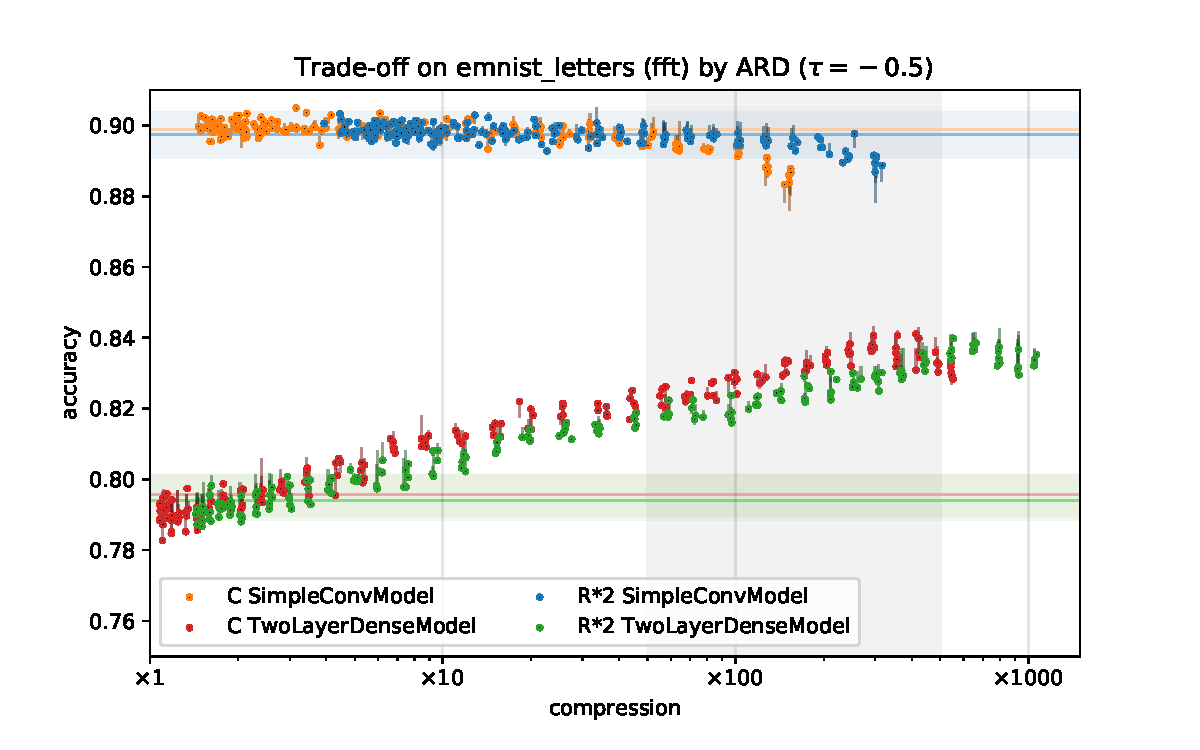
\includegraphics[width=\columnwidth]{figure__mnist-like__trade-off/appendix__cmp__ARD__emnist_letters__fft__-0.5.pdf}
  \end{subfigure}%
  \begin{subfigure}[b]{0.5\columnwidth}
    \centering
    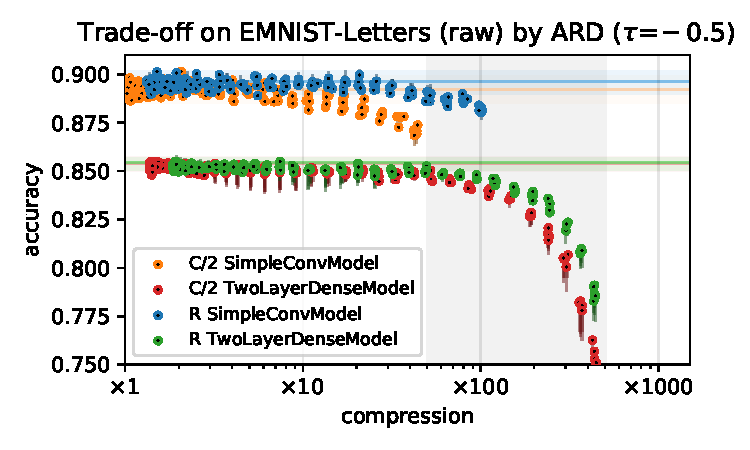
\includegraphics[width=\columnwidth]{figure__mnist-like__trade-off/appendix__cmp__ARD__emnist_letters__raw__-0.5.pdf}
  \end{subfigure} \\ %
  \begin{subfigure}[b]{0.5\columnwidth}
    \centering
    % used in main text
    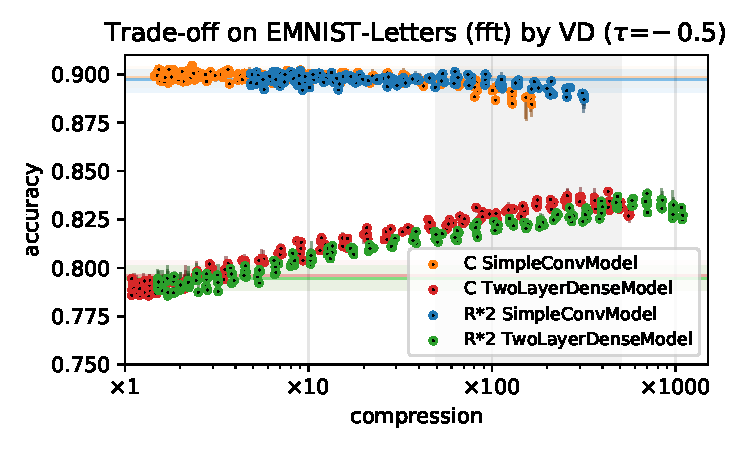
\includegraphics[width=\columnwidth]{figure__mnist-like__trade-off/appendix__cmp__VD__emnist_letters__fft__-0.5.pdf}
  \end{subfigure}%
  \begin{subfigure}[b]{0.5\columnwidth}
    \centering
    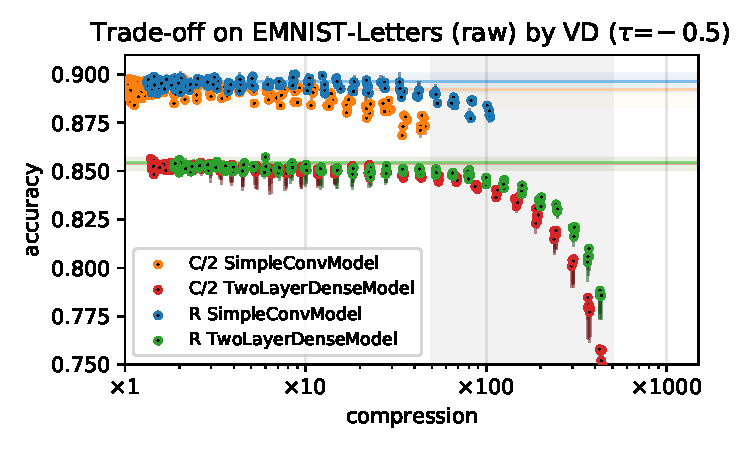
\includegraphics[width=\columnwidth]{figure__mnist-like__trade-off/appendix__cmp__VD__emnist_letters__raw__-0.5.pdf}
  \end{subfigure} \\ %
  \begin{subfigure}[b]{0.5\columnwidth}
    \centering
    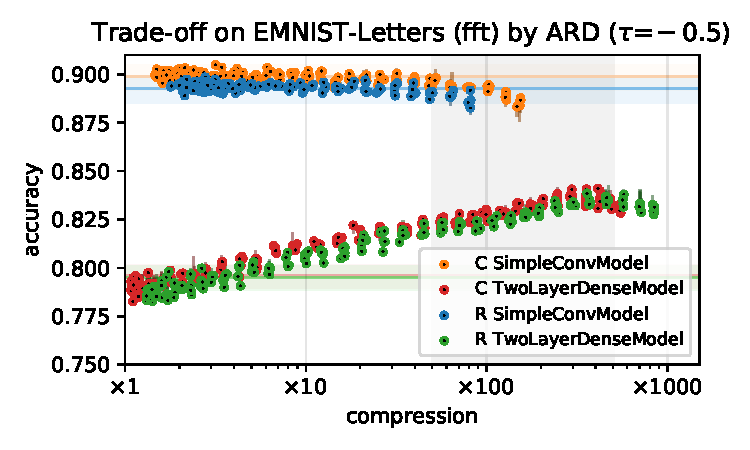
\includegraphics[width=\columnwidth]{figure__mnist-like__trade-off/appendix__ARD__emnist_letters__fft__-0.5.pdf}
  \end{subfigure}%
  \begin{subfigure}[b]{0.5\columnwidth}
    \centering
    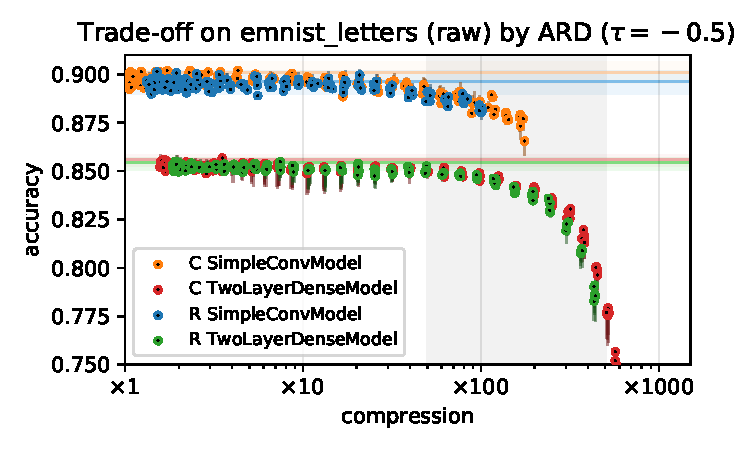
\includegraphics[width=\columnwidth]{figure__mnist-like__trade-off/appendix__ARD__emnist_letters__raw__-0.5.pdf}
  \end{subfigure} \\ %
  \begin{subfigure}[b]{0.5\columnwidth}
    \centering
    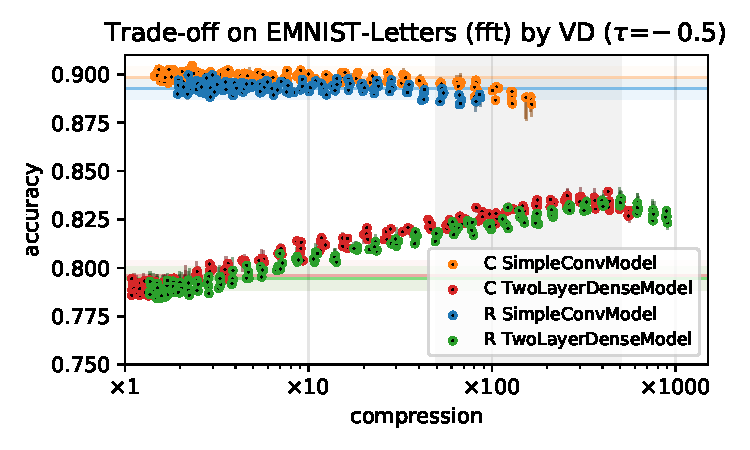
\includegraphics[width=\columnwidth]{figure__mnist-like__trade-off/appendix__VD__emnist_letters__fft__-0.5.pdf}
  \end{subfigure}%
  \begin{subfigure}[b]{0.5\columnwidth}
    \centering
    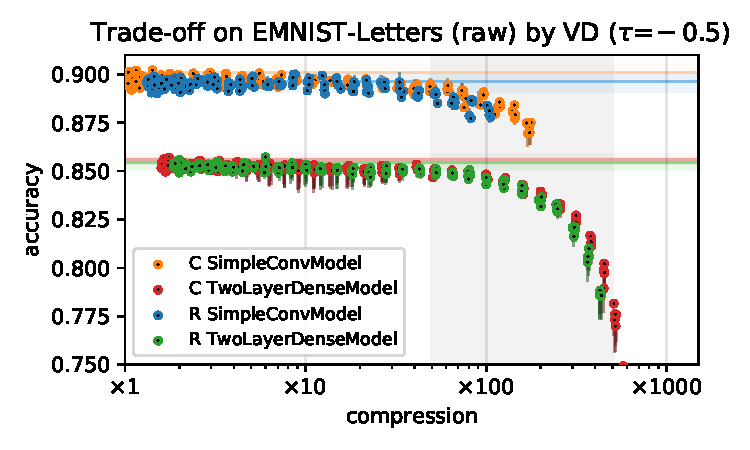
\includegraphics[width=\columnwidth]{figure__mnist-like__trade-off/appendix__VD__emnist_letters__raw__-0.5.pdf}
  \end{subfigure}
  \caption{%
    \texttt{emnist\_letters}:
      \texttt{fft} (left), \texttt{raw} (right).
      Models on rows 1 \& 2 are incomparable: (left $2\real / \cplx$), (right $\real / \tfrac12\cplx$).
      Rows 3 \& 4 feature $\real / \cplx$ models.
    % ARD method for $\real$ and $\cplx$ models using Fourier features.
  }
  % \label{fig:appendix__mnist-like__trade-off__emnist_letters}
\end{figure}

\begin{figure}[b]
  \centering
  \begin{subfigure}[b]{0.5\columnwidth}
    \centering
    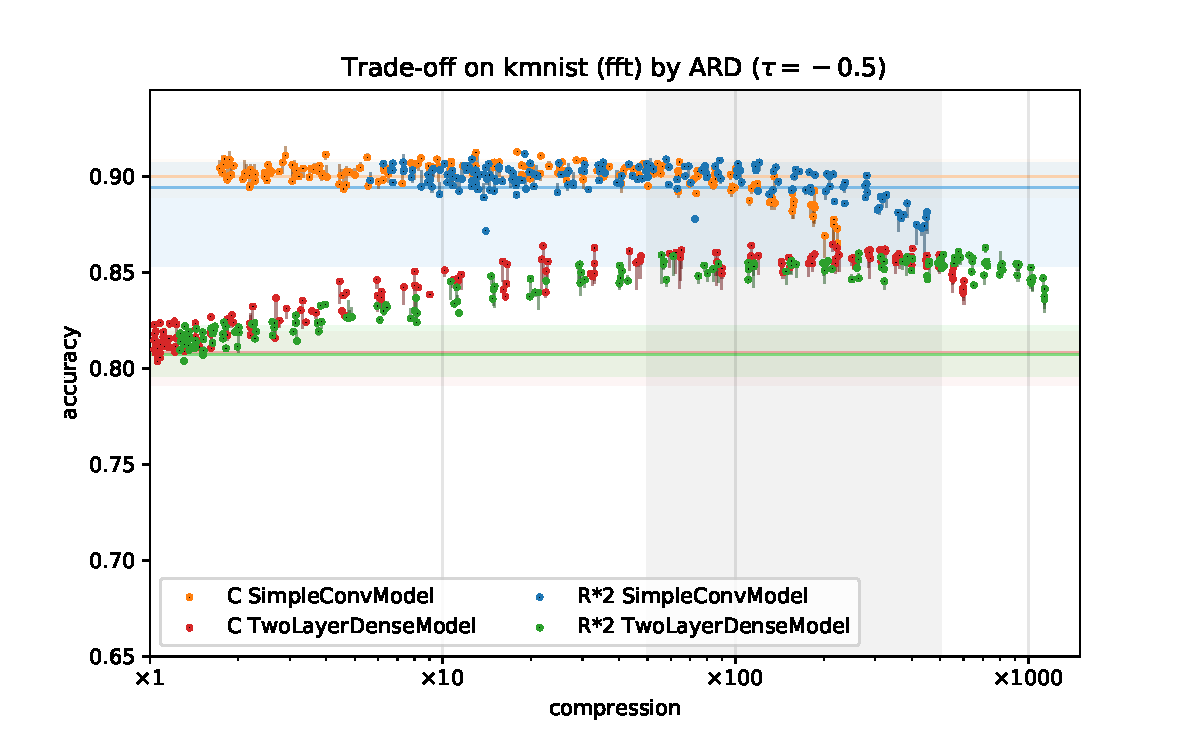
\includegraphics[width=\columnwidth]{figure__mnist-like__trade-off/appendix__cmp__ARD__kmnist__fft__-0.5.pdf}
  \end{subfigure}%
  \begin{subfigure}[b]{0.5\columnwidth}
    \centering
    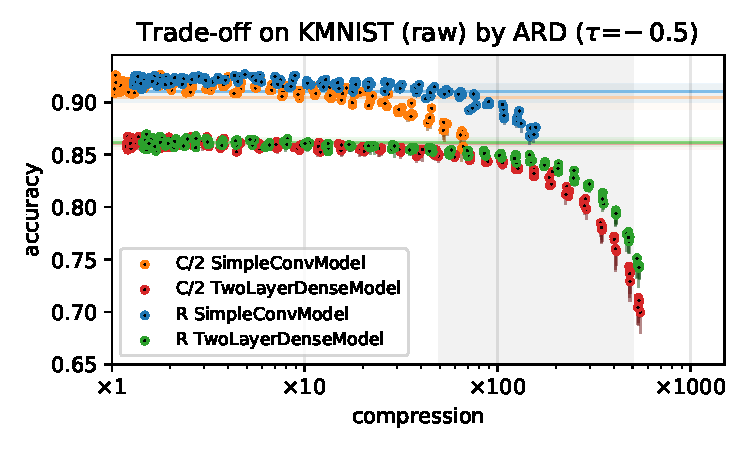
\includegraphics[width=\columnwidth]{figure__mnist-like__trade-off/appendix__cmp__ARD__kmnist__raw__-0.5.pdf}
  \end{subfigure} \\ %
  \begin{subfigure}[b]{0.5\columnwidth}
    \centering
    % used in main text
    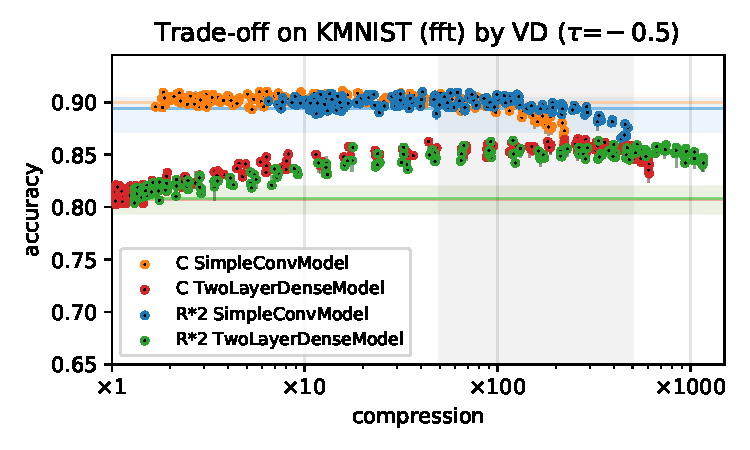
\includegraphics[width=\columnwidth]{figure__mnist-like__trade-off/appendix__cmp__VD__kmnist__fft__-0.5.pdf}
  \end{subfigure}%
  \begin{subfigure}[b]{0.5\columnwidth}
    \centering
    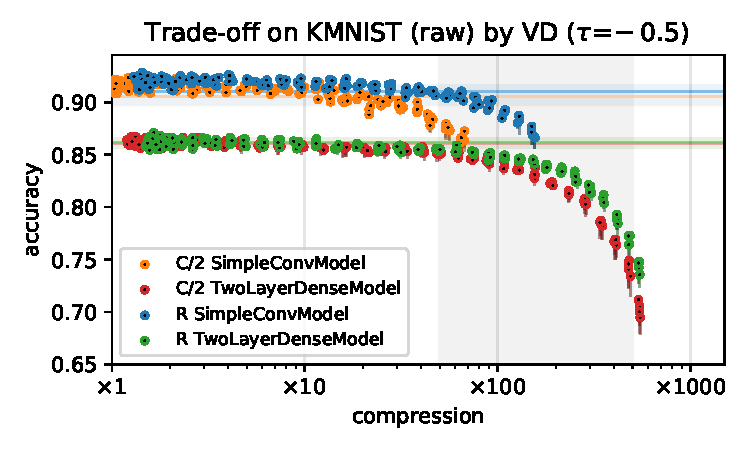
\includegraphics[width=\columnwidth]{figure__mnist-like__trade-off/appendix__cmp__VD__kmnist__raw__-0.5.pdf}
  \end{subfigure} \\ %
  \begin{subfigure}[b]{0.5\columnwidth}
    \centering
    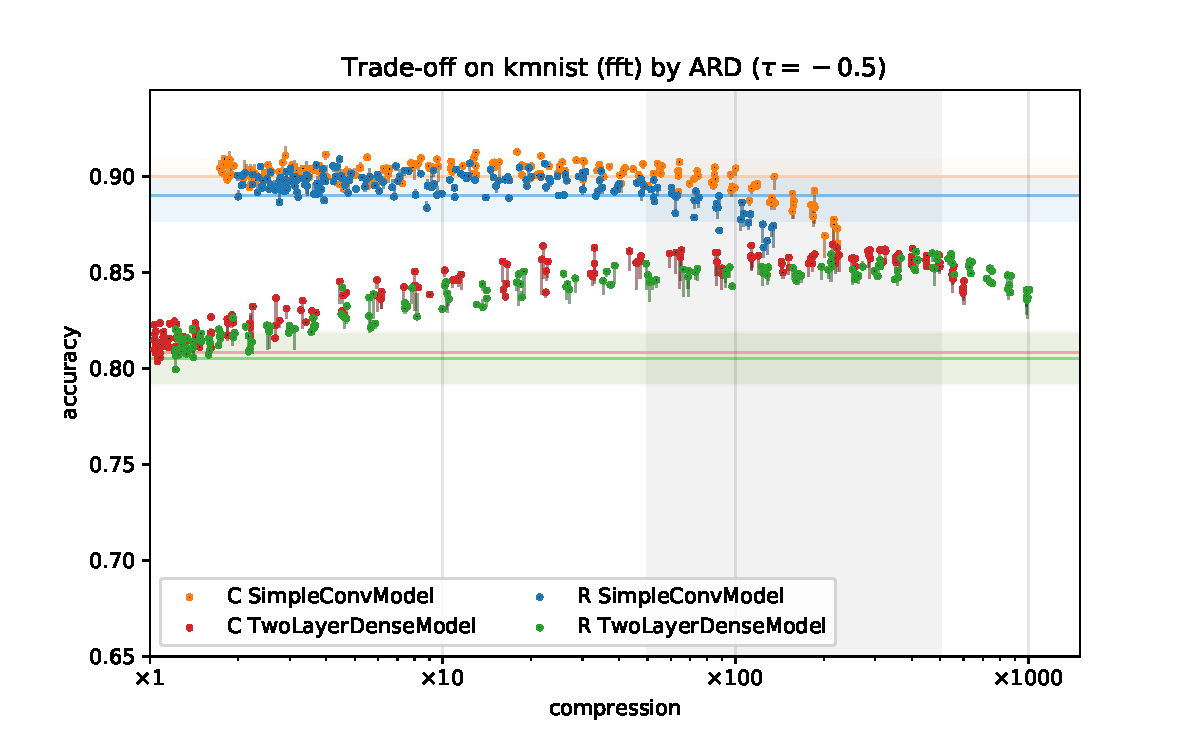
\includegraphics[width=\columnwidth]{figure__mnist-like__trade-off/appendix__ARD__kmnist__fft__-0.5.pdf}
  \end{subfigure}%
  \begin{subfigure}[b]{0.5\columnwidth}
    \centering
    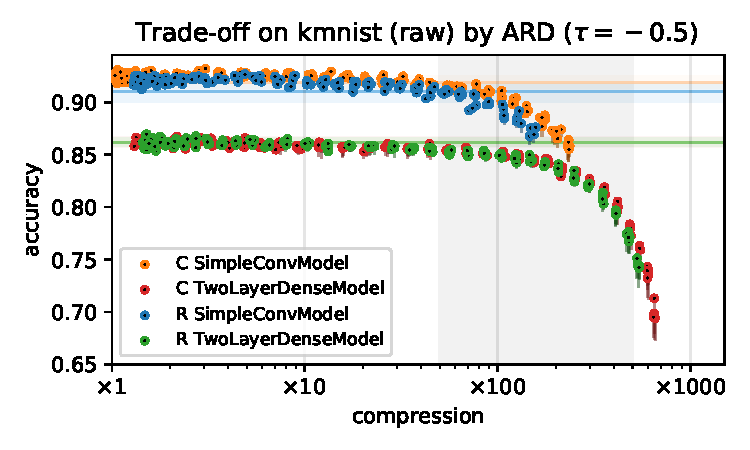
\includegraphics[width=\columnwidth]{figure__mnist-like__trade-off/appendix__ARD__kmnist__raw__-0.5.pdf}
  \end{subfigure} \\ %
  \begin{subfigure}[b]{0.5\columnwidth}
    \centering
    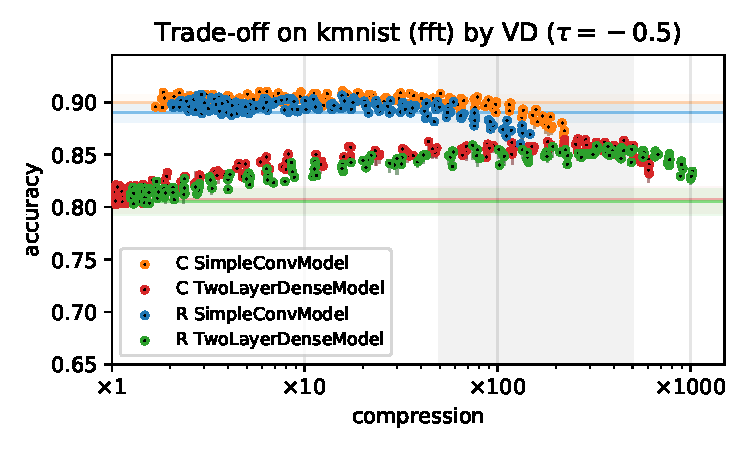
\includegraphics[width=\columnwidth]{figure__mnist-like__trade-off/appendix__VD__kmnist__fft__-0.5.pdf}
  \end{subfigure}%
  \begin{subfigure}[b]{0.5\columnwidth}
    \centering
    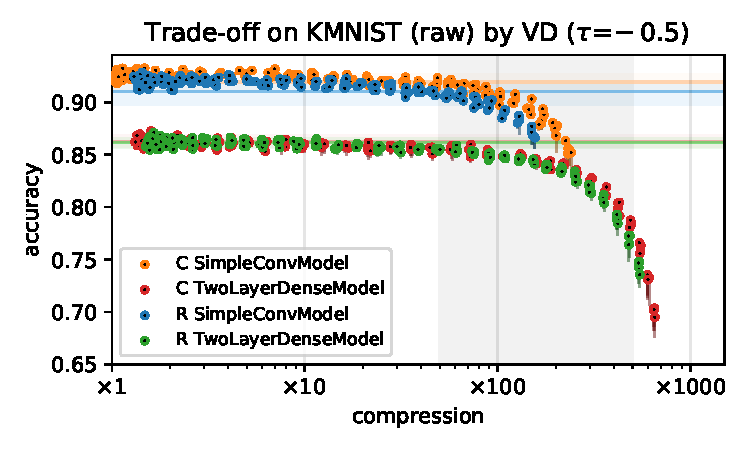
\includegraphics[width=\columnwidth]{figure__mnist-like__trade-off/appendix__VD__kmnist__raw__-0.5.pdf}
  \end{subfigure}
  \caption{%
    \texttt{kmnist}:
      \texttt{fft} (left), \texttt{raw} (right).
      Models on rows 1 \& 2 are incomparable: (left $2\real / \cplx$), (right $\real / \tfrac12\cplx$).
      Rows 3 \& 4 feature $\real / \cplx$ models.
    % VD method for $\real$ and $\cplx$ models using Fourier features.
  }
  % \label{fig:appendix__mnist-like__trade-off__kmnist}
\end{figure}

\begin{figure}[b]
  \centering
  \begin{subfigure}[b]{0.5\columnwidth}
    \centering
    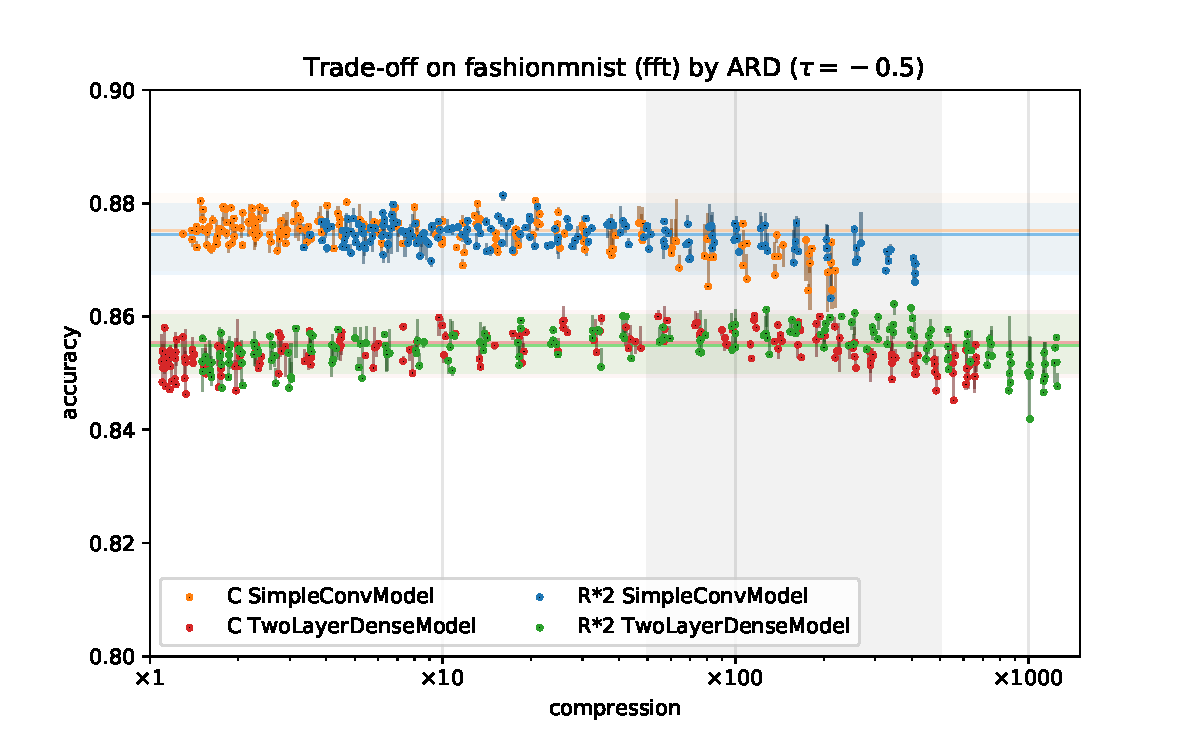
\includegraphics[width=\columnwidth]{figure__mnist-like__trade-off/appendix__cmp__ARD__fashionmnist__fft__-0.5.pdf}
  \end{subfigure}%
  \begin{subfigure}[b]{0.5\columnwidth}
    \centering
    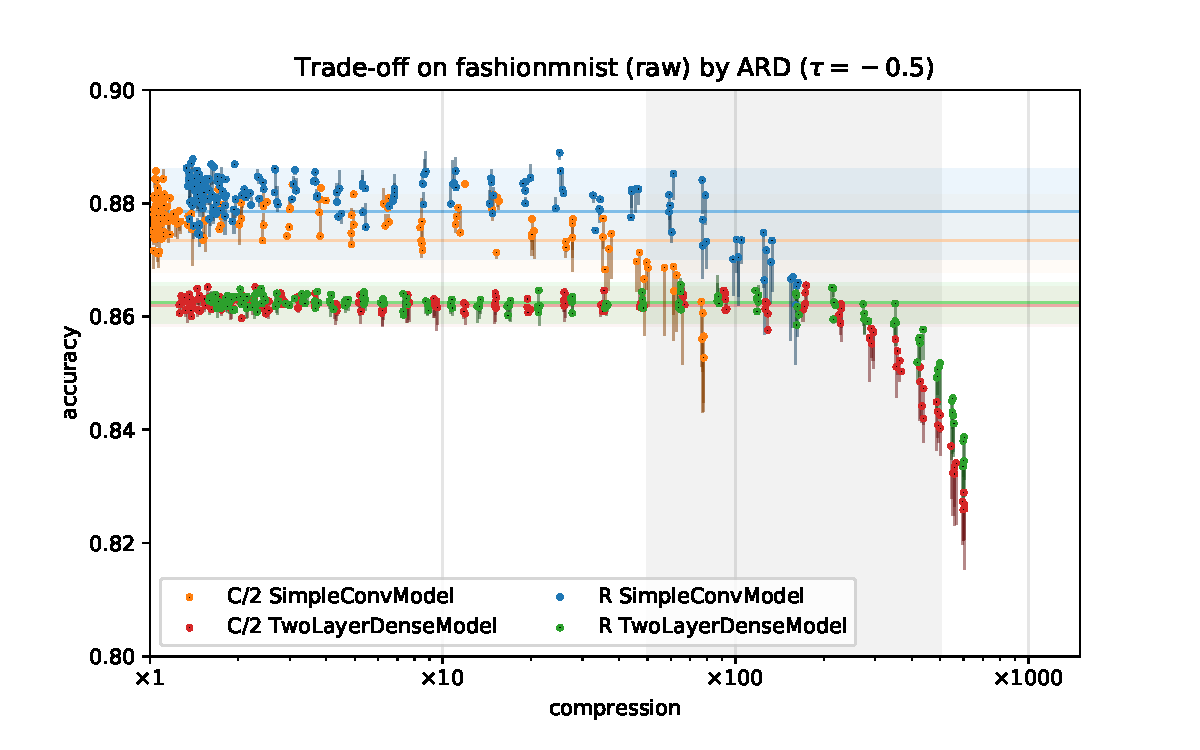
\includegraphics[width=\columnwidth]{figure__mnist-like__trade-off/appendix__cmp__ARD__fashionmnist__raw__-0.5.pdf}
  \end{subfigure} \\%
  \begin{subfigure}[b]{0.5\columnwidth}
    \centering
    % used in main text
    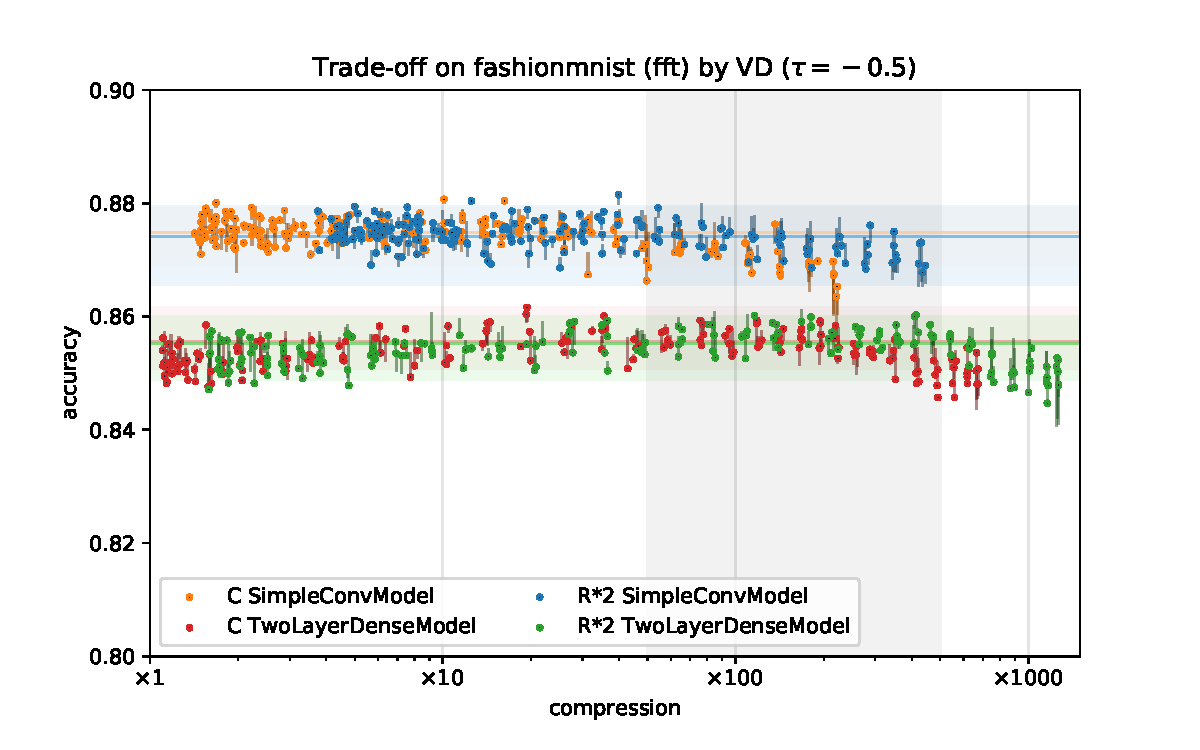
\includegraphics[width=\columnwidth]{figure__mnist-like__trade-off/appendix__cmp__VD__fashionmnist__fft__-0.5.pdf}
  \end{subfigure}%
  \begin{subfigure}[b]{0.5\columnwidth}
    \centering
    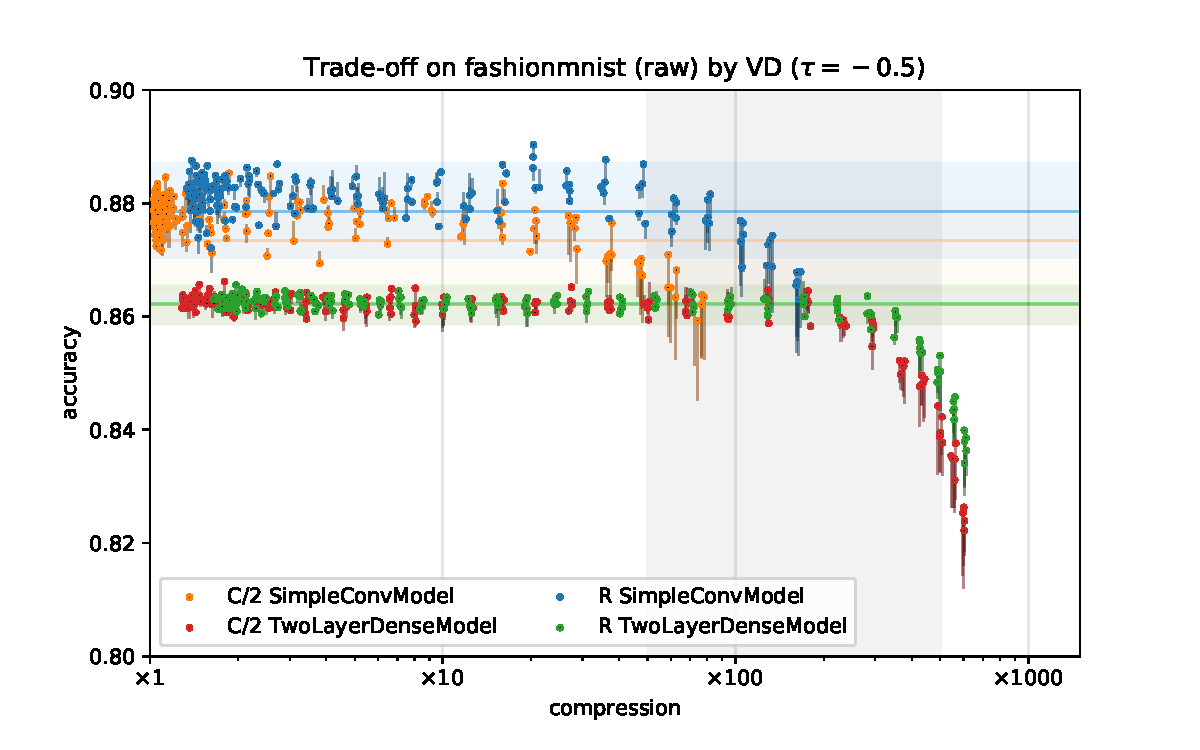
\includegraphics[width=\columnwidth]{figure__mnist-like__trade-off/appendix__cmp__VD__fashionmnist__raw__-0.5.pdf}
  \end{subfigure} \\%
  \begin{subfigure}[b]{0.5\columnwidth}
    \centering
    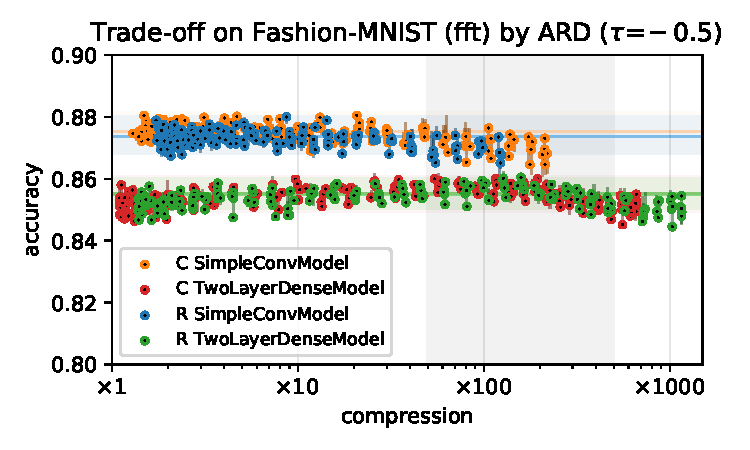
\includegraphics[width=\columnwidth]{figure__mnist-like__trade-off/appendix__ARD__fashionmnist__fft__-0.5.pdf}
  \end{subfigure}%
  \begin{subfigure}[b]{0.5\columnwidth}
    \centering
    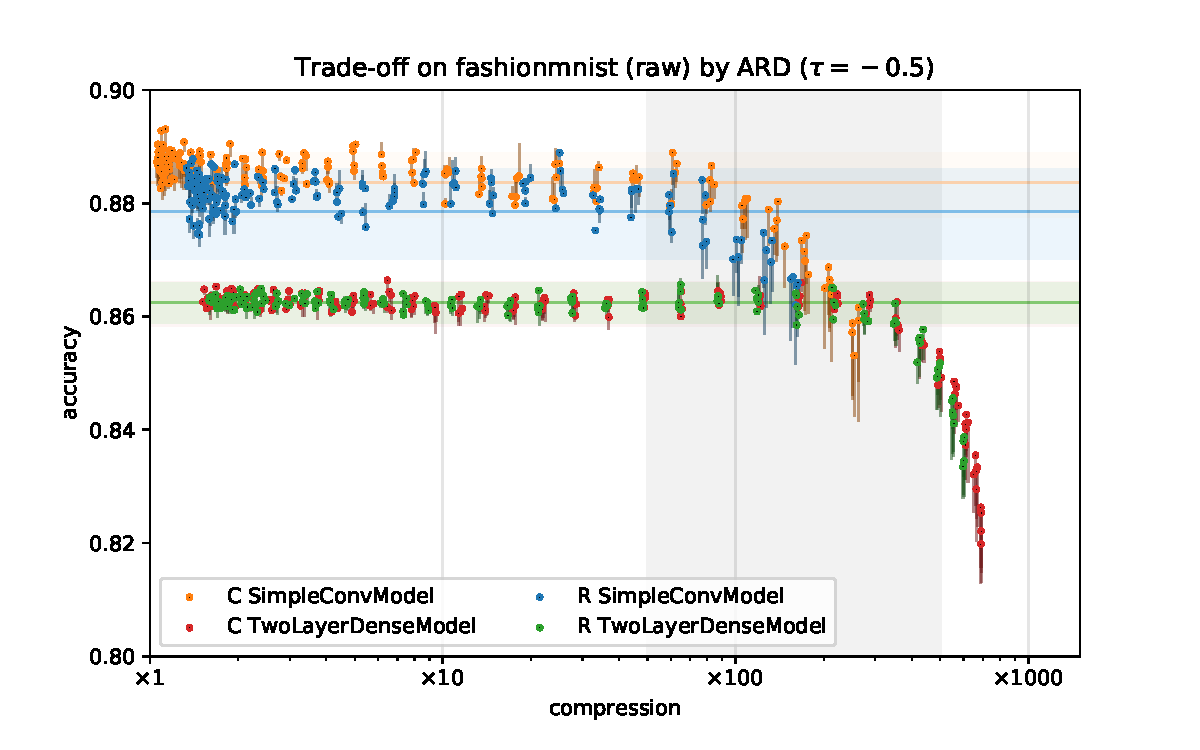
\includegraphics[width=\columnwidth]{figure__mnist-like__trade-off/appendix__ARD__fashionmnist__raw__-0.5.pdf}
  \end{subfigure} \\ %
  \begin{subfigure}[b]{0.5\columnwidth}
    \centering
    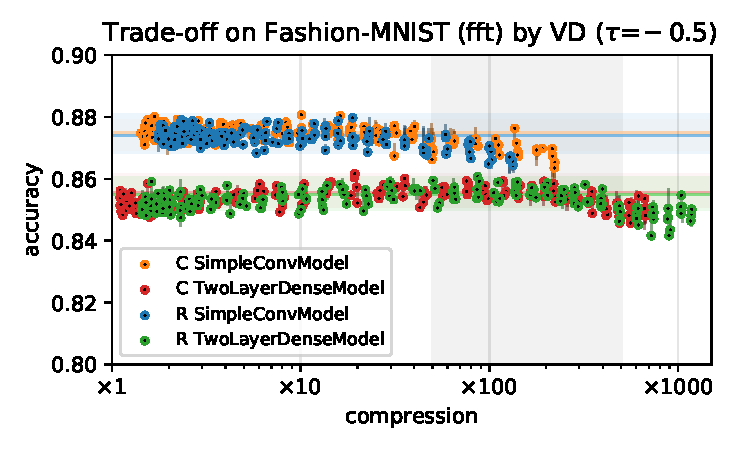
\includegraphics[width=\columnwidth]{figure__mnist-like__trade-off/appendix__VD__fashionmnist__fft__-0.5.pdf}
  \end{subfigure}%
  \begin{subfigure}[b]{0.5\columnwidth}
    \centering
    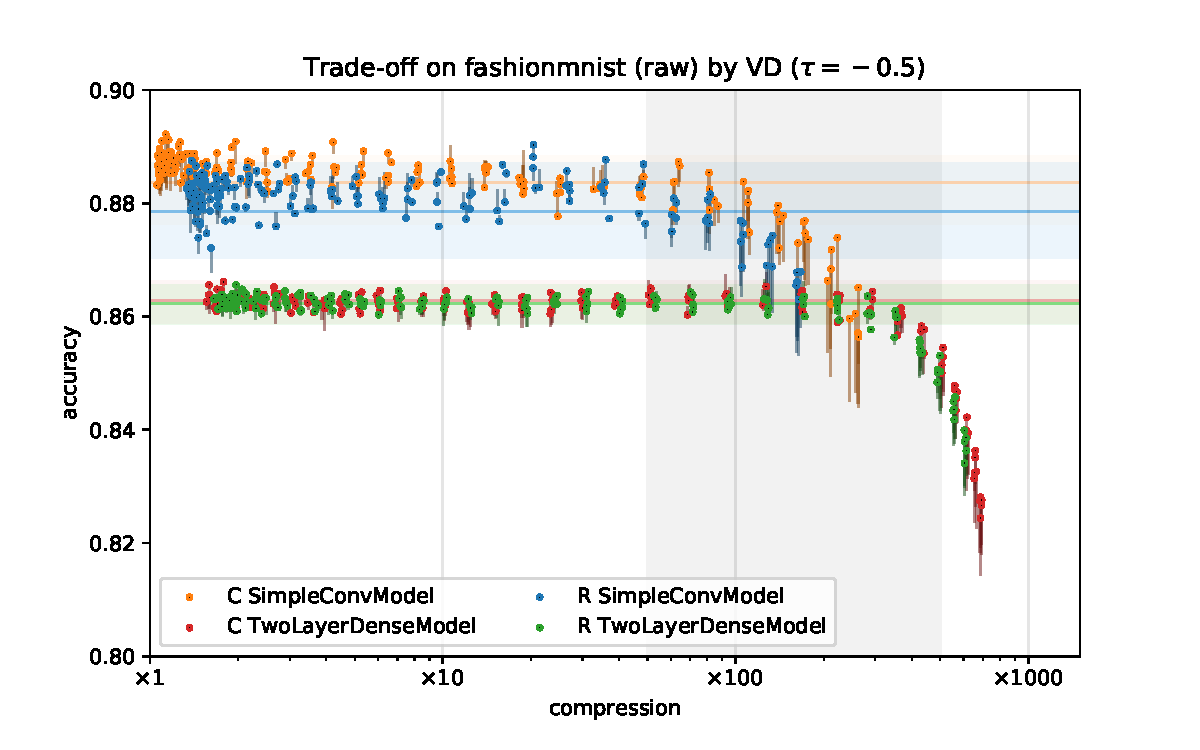
\includegraphics[width=\columnwidth]{figure__mnist-like__trade-off/appendix__VD__fashionmnist__raw__-0.5.pdf}
  \end{subfigure}
  \caption{%
    \texttt{fashionmnist}:
      \texttt{fft} (left), \texttt{raw} (right).
      Models on rows 1 \& 2 are incomparable: (left $2\real / \cplx$), (right $\real / \tfrac12\cplx$).
      Rows 3 \& 4 feature $\real / \cplx$ models.
    % ARD method for $\real$ and $\cplx$ models using raw features.
  }
  % \label{fig:appendix__mnist-like__trade-off__fashionmnist}
\end{figure}

\begin{figure}[b]
  \centering
  \begin{subfigure}[b]{0.5\columnwidth}
    \centering
    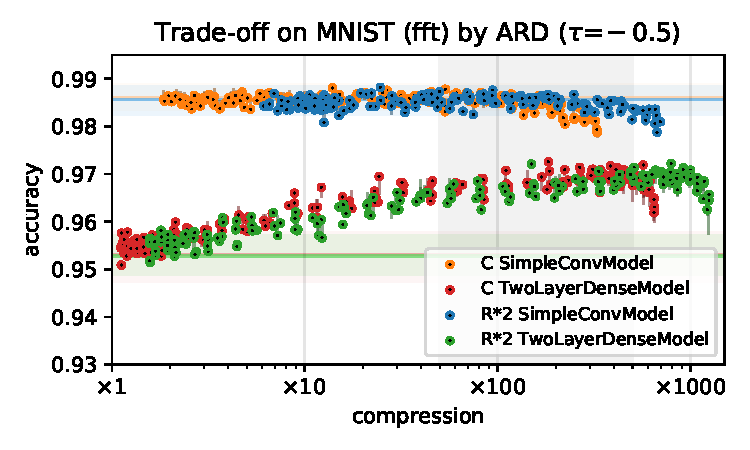
\includegraphics[width=\columnwidth]{figure__mnist-like__trade-off/appendix__cmp__ARD__mnist__fft__-0.5.pdf}
  \end{subfigure}%
  \begin{subfigure}[b]{0.5\columnwidth}
    \centering
    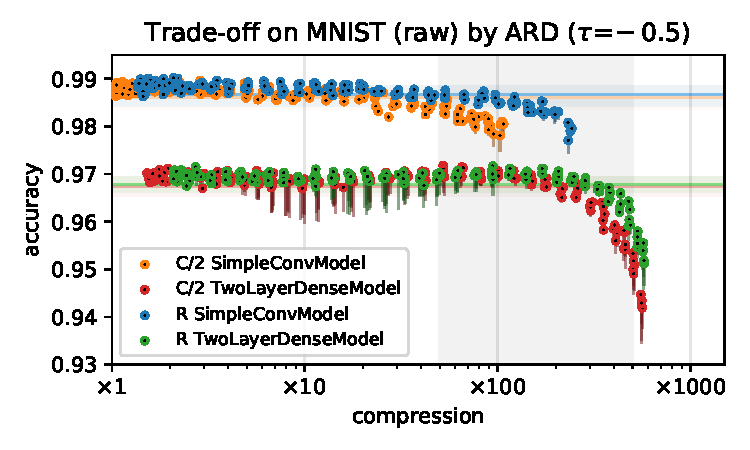
\includegraphics[width=\columnwidth]{figure__mnist-like__trade-off/appendix__cmp__ARD__mnist__raw__-0.5.pdf}
  \end{subfigure} \\%
  \begin{subfigure}[b]{0.5\columnwidth}
    \centering
    % used in main text
    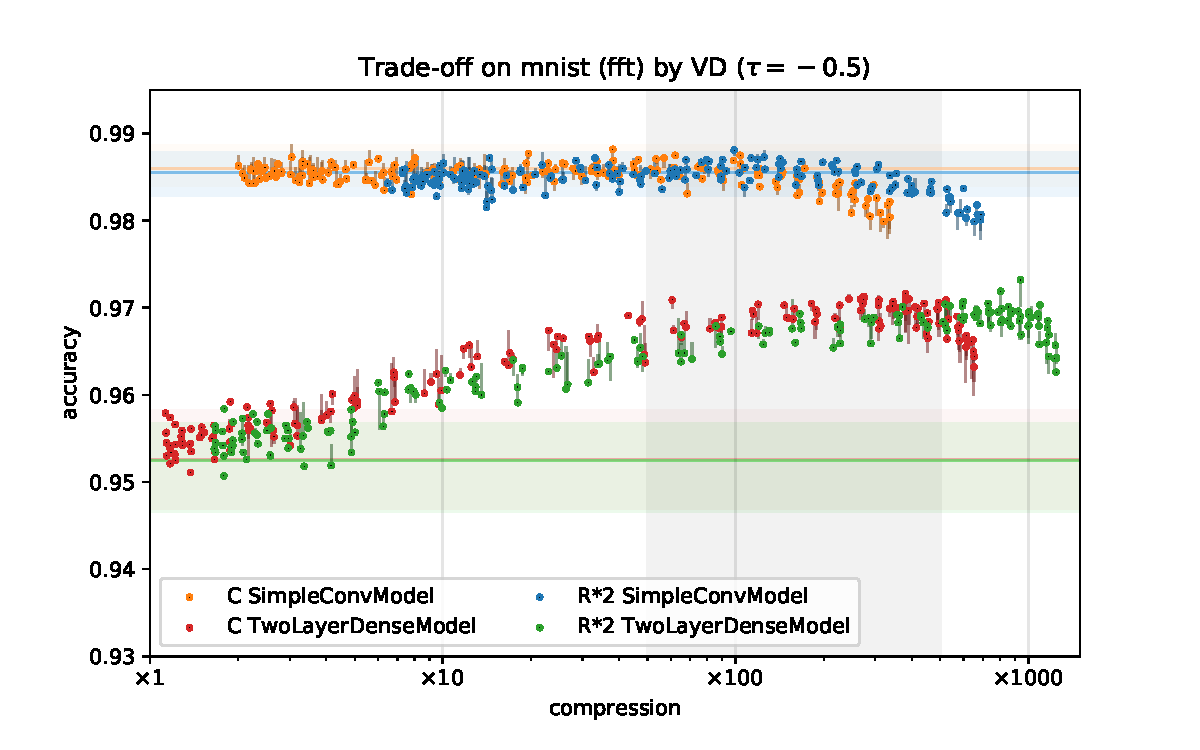
\includegraphics[width=\columnwidth]{figure__mnist-like__trade-off/appendix__cmp__VD__mnist__fft__-0.5.pdf}
  \end{subfigure}%
  \begin{subfigure}[b]{0.5\columnwidth}
    \centering
    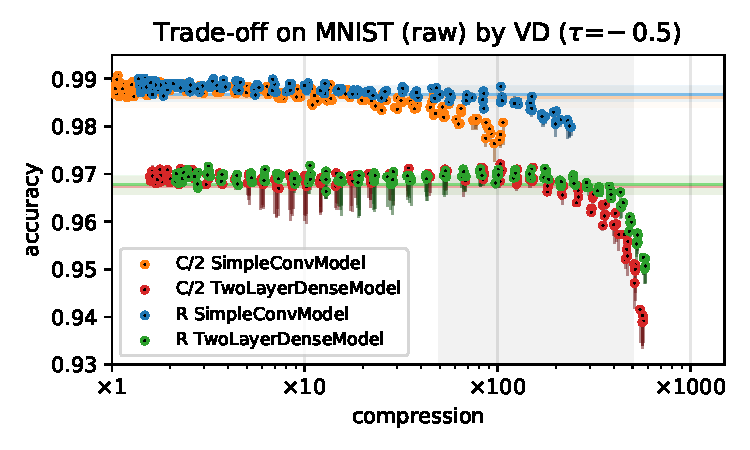
\includegraphics[width=\columnwidth]{figure__mnist-like__trade-off/appendix__cmp__VD__mnist__raw__-0.5.pdf}
  \end{subfigure} \\%
  \begin{subfigure}[b]{0.5\columnwidth}
    \centering
    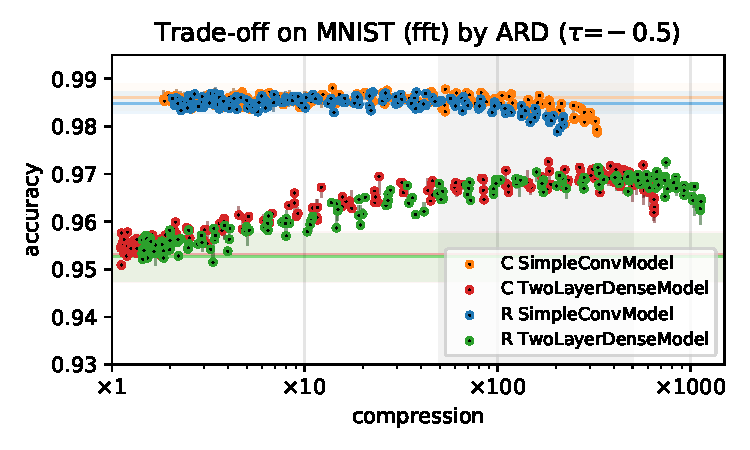
\includegraphics[width=\columnwidth]{figure__mnist-like__trade-off/appendix__ARD__mnist__fft__-0.5.pdf}
  \end{subfigure}%
  \begin{subfigure}[b]{0.5\columnwidth}
    \centering
    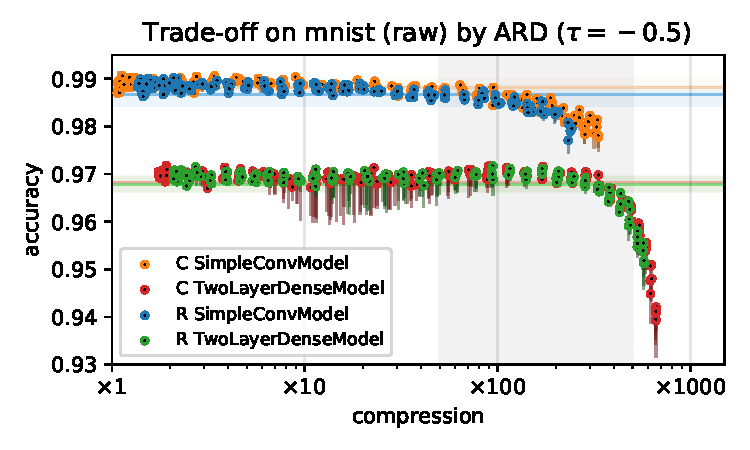
\includegraphics[width=\columnwidth]{figure__mnist-like__trade-off/appendix__ARD__mnist__raw__-0.5.pdf}
  \end{subfigure} \\ %
  \begin{subfigure}[b]{0.5\columnwidth}
    \centering
    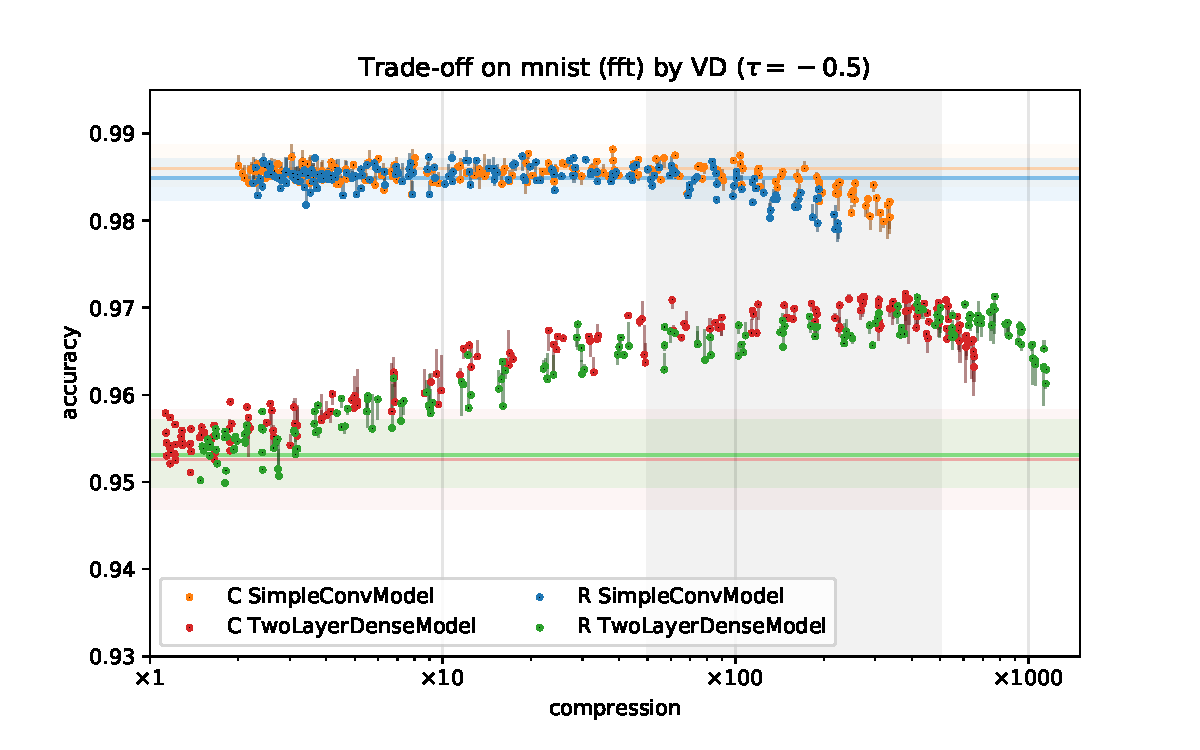
\includegraphics[width=\columnwidth]{figure__mnist-like__trade-off/appendix__VD__mnist__fft__-0.5.pdf}
  \end{subfigure}%
  \begin{subfigure}[b]{0.5\columnwidth}
    \centering
    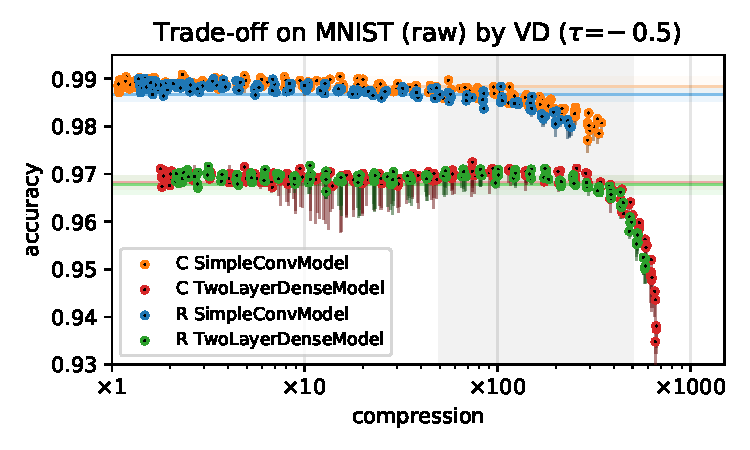
\includegraphics[width=\columnwidth]{figure__mnist-like__trade-off/appendix__VD__mnist__raw__-0.5.pdf}
  \end{subfigure}
  \caption{%
    \texttt{mnist}:
      \texttt{fft} (left), \texttt{raw} (right).
      Models on rows 1 \& 2 are incomparable: (left $2\real / \cplx$), (right $\real / \tfrac12\cplx$).
      Rows 3 \& 4 feature $\real / \cplx$ models.
    % VD method for $\real$ and $\cplx$ models using raw features.
  }
  % \label{fig:appendix__mnist-like__trade-off__mnist}
\end{figure}

\begin{figure}[b]
  \centering
  \begin{subfigure}[b]{0.5\columnwidth}
    \centering
    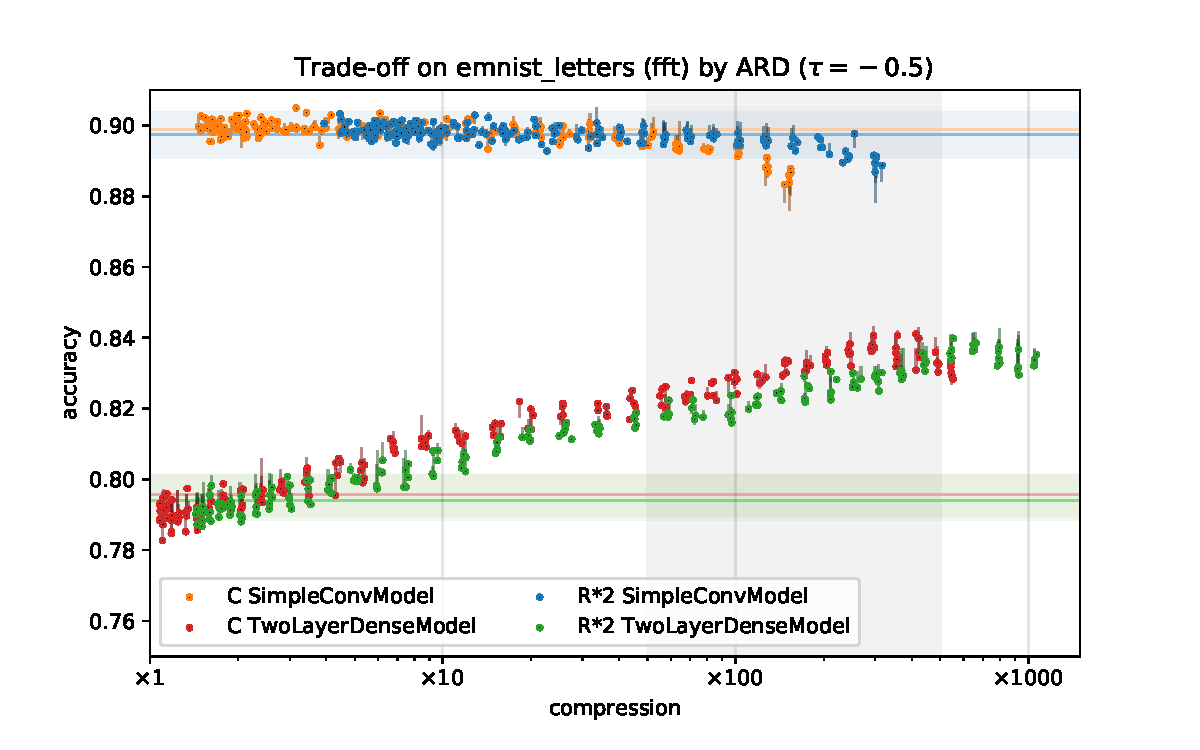
\includegraphics[width=\columnwidth]{figure__mnist-like__trade-off/appendix__cmp__ARD__emnist_letters__fft__-0.5.pdf}
  \end{subfigure}%
  \begin{subfigure}[b]{0.5\columnwidth}
    \centering
    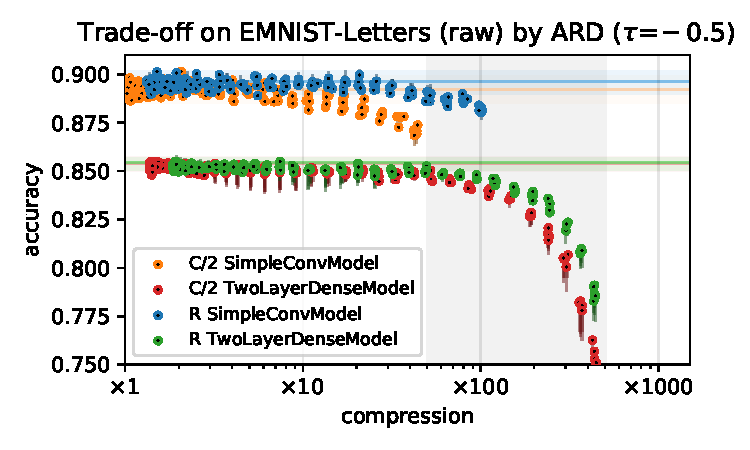
\includegraphics[width=\columnwidth]{figure__mnist-like__trade-off/appendix__cmp__ARD__emnist_letters__raw__-0.5.pdf}
  \end{subfigure} \\ %
  \begin{subfigure}[b]{0.5\columnwidth}
    \centering
    % used in main text
    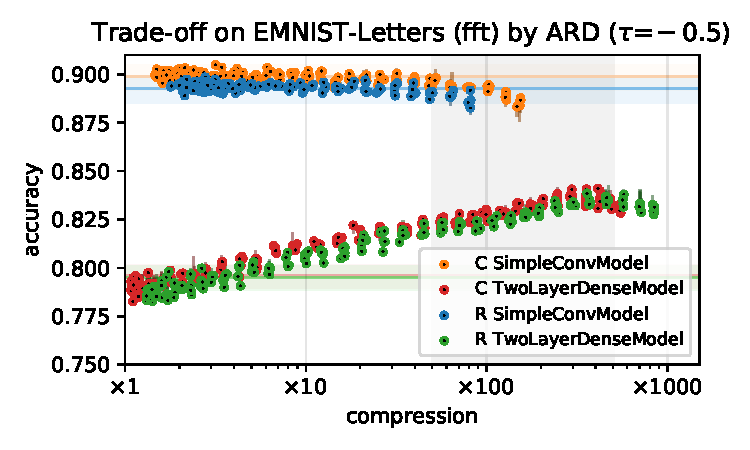
\includegraphics[width=\columnwidth]{figure__mnist-like__trade-off/appendix__ARD__emnist_letters__fft__-0.5.pdf}
  \end{subfigure}%
  \begin{subfigure}[b]{0.5\columnwidth}
    \centering
    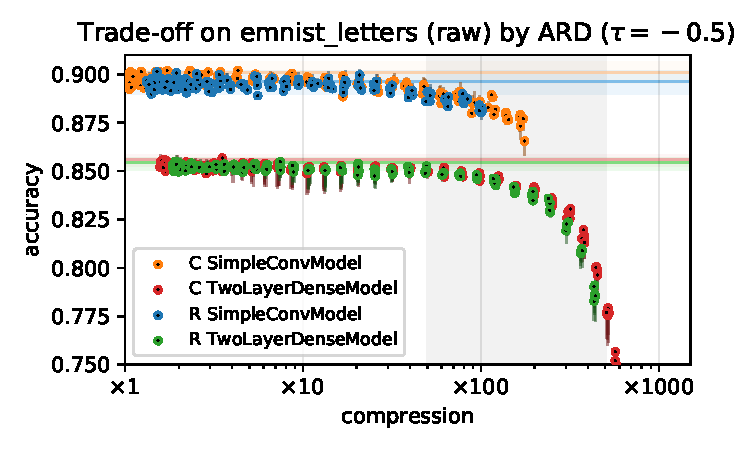
\includegraphics[width=\columnwidth]{figure__mnist-like__trade-off/appendix__ARD__emnist_letters__raw__-0.5.pdf}
  \end{subfigure} \\ %
  \begin{subfigure}[b]{0.5\columnwidth}
    \centering
    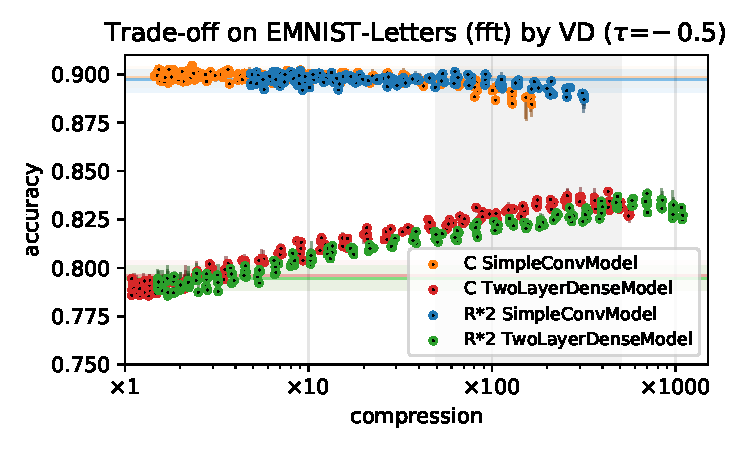
\includegraphics[width=\columnwidth]{figure__mnist-like__trade-off/appendix__cmp__VD__emnist_letters__fft__-0.5.pdf}
  \end{subfigure}%
  \begin{subfigure}[b]{0.5\columnwidth}
    \centering
    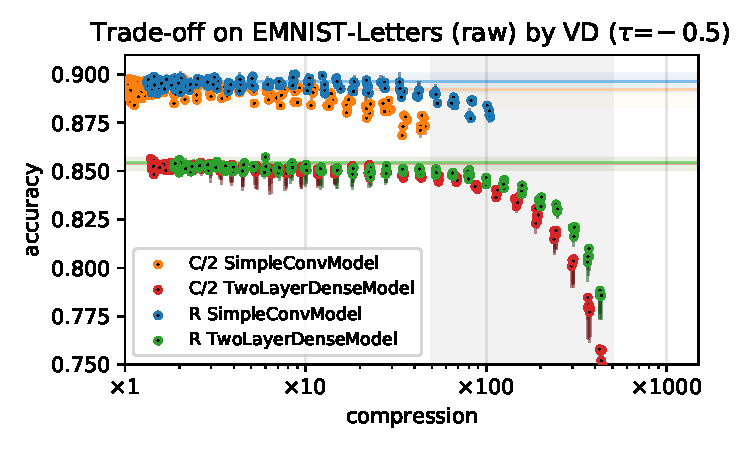
\includegraphics[width=\columnwidth]{figure__mnist-like__trade-off/appendix__cmp__VD__emnist_letters__raw__-0.5.pdf}
  \end{subfigure} \\ %
  \begin{subfigure}[b]{0.5\columnwidth}
    \centering
    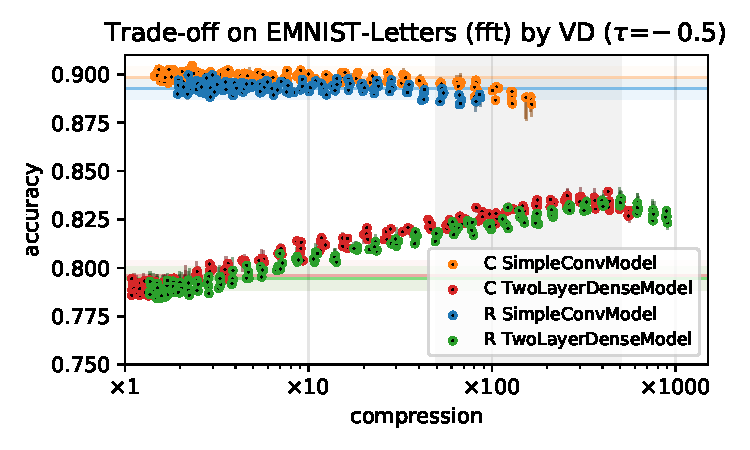
\includegraphics[width=\columnwidth]{figure__mnist-like__trade-off/appendix__VD__emnist_letters__fft__-0.5.pdf}
  \end{subfigure}%
  \begin{subfigure}[b]{0.5\columnwidth}
    \centering
    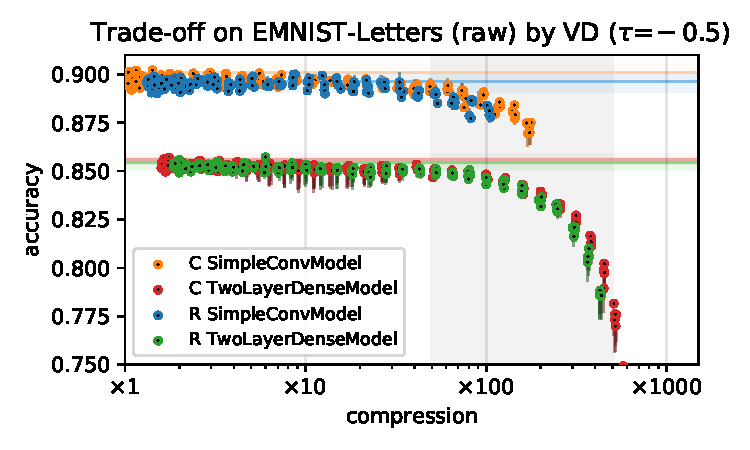
\includegraphics[width=\columnwidth]{figure__mnist-like__trade-off/appendix__VD__emnist_letters__raw__-0.5.pdf}
  \end{subfigure}
  \caption{%
    \texttt{emnist\_letters}:
      \texttt{fft} (left), \texttt{raw} (right).
      Models on rows 1 \& 2 are incomparable: (left $2\real / \cplx$), (right $\real / \tfrac12\cplx$).
      Rows 3 \& 4 feature $\real / \cplx$ models.
    % ARD method for $\real$ and $\cplx$ models using Fourier features.
  }
  % \label{fig:appendix__mnist-like__trade-off__emnist_letters}
\end{figure}

\begin{figure}[b]
  \centering
  \begin{subfigure}[b]{0.5\columnwidth}
    \centering
    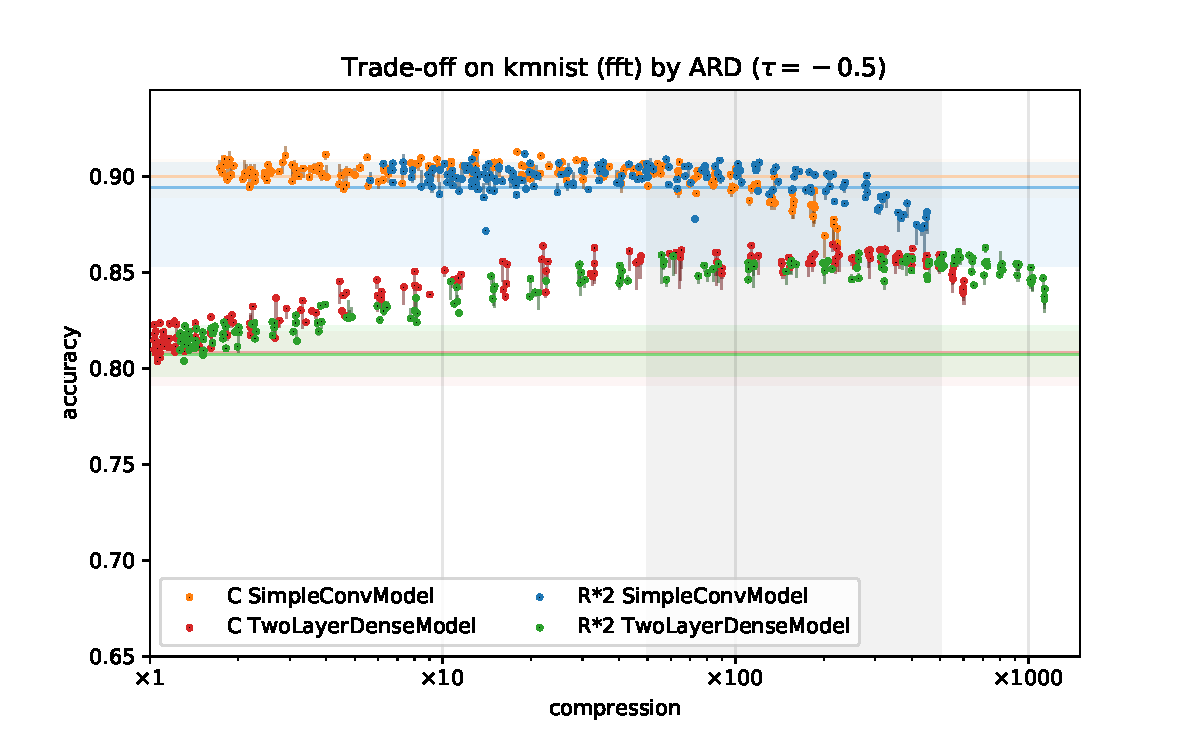
\includegraphics[width=\columnwidth]{figure__mnist-like__trade-off/appendix__cmp__ARD__kmnist__fft__-0.5.pdf}
  \end{subfigure}%
  \begin{subfigure}[b]{0.5\columnwidth}
    \centering
    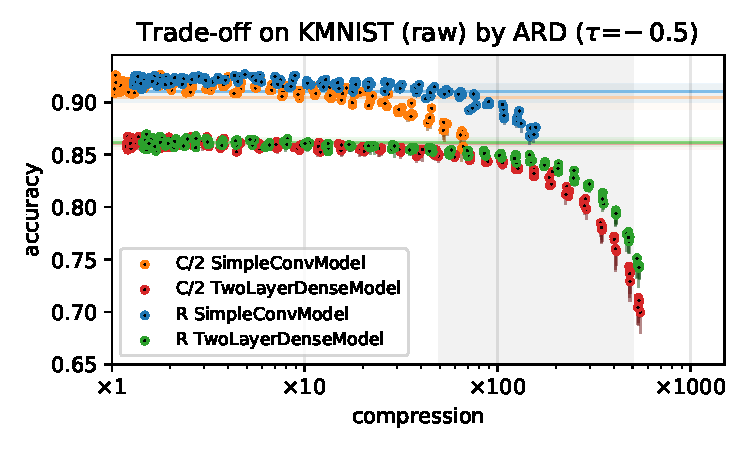
\includegraphics[width=\columnwidth]{figure__mnist-like__trade-off/appendix__cmp__ARD__kmnist__raw__-0.5.pdf}
  \end{subfigure} \\ %
  \begin{subfigure}[b]{0.5\columnwidth}
    \centering
    % used in main text
    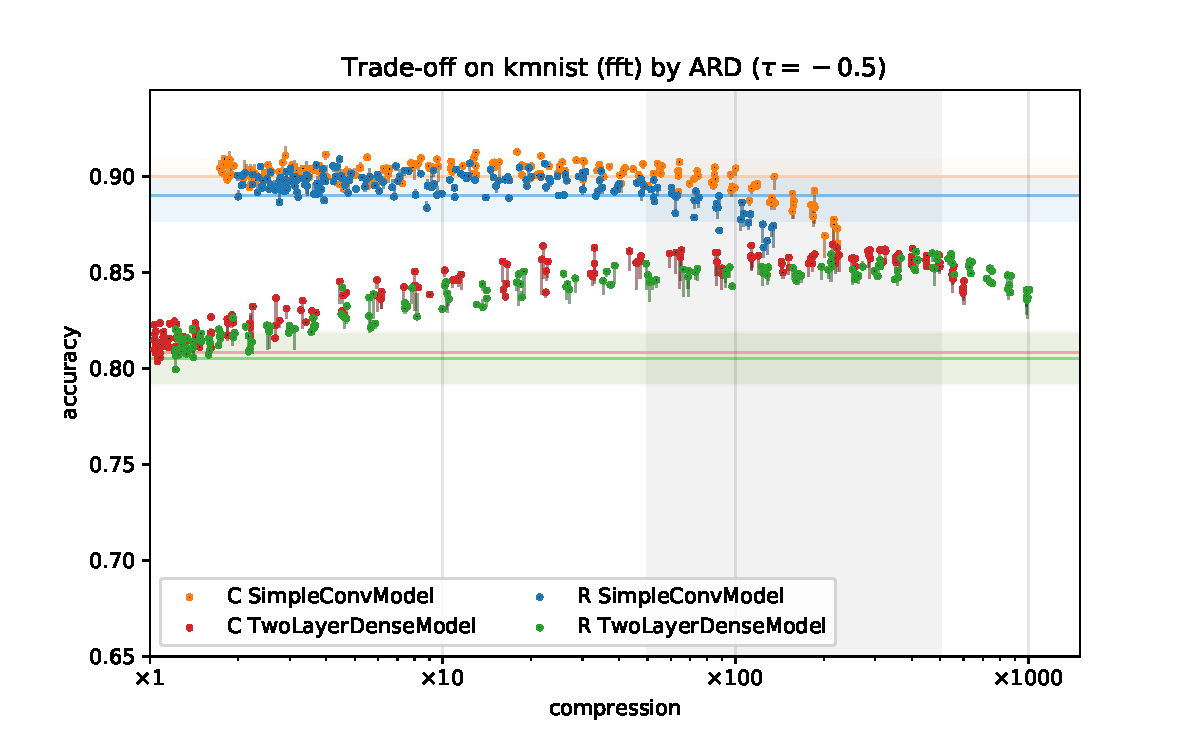
\includegraphics[width=\columnwidth]{figure__mnist-like__trade-off/appendix__ARD__kmnist__fft__-0.5.pdf}
  \end{subfigure}%
  \begin{subfigure}[b]{0.5\columnwidth}
    \centering
    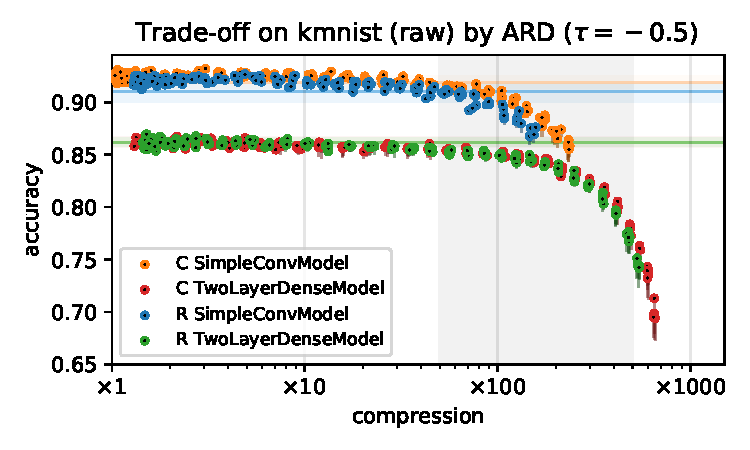
\includegraphics[width=\columnwidth]{figure__mnist-like__trade-off/appendix__ARD__kmnist__raw__-0.5.pdf}
  \end{subfigure} \\ %
  \begin{subfigure}[b]{0.5\columnwidth}
    \centering
    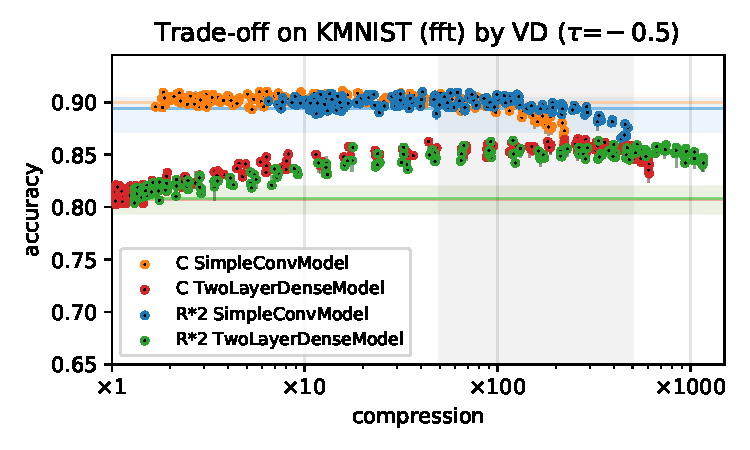
\includegraphics[width=\columnwidth]{figure__mnist-like__trade-off/appendix__cmp__VD__kmnist__fft__-0.5.pdf}
  \end{subfigure}%
  \begin{subfigure}[b]{0.5\columnwidth}
    \centering
    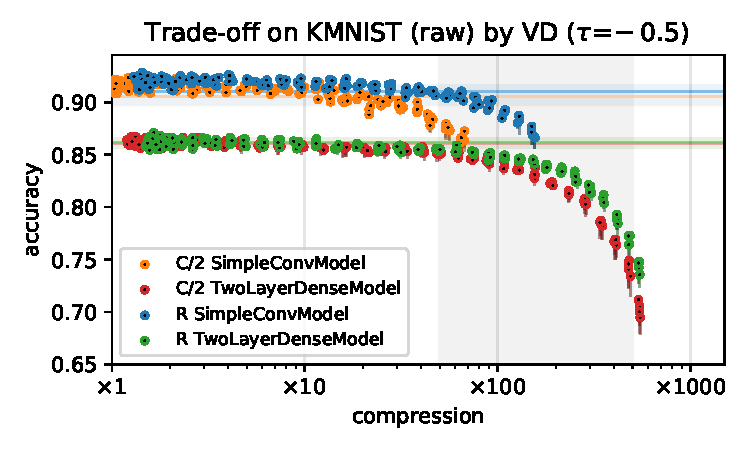
\includegraphics[width=\columnwidth]{figure__mnist-like__trade-off/appendix__cmp__VD__kmnist__raw__-0.5.pdf}
  \end{subfigure} \\ %
  \begin{subfigure}[b]{0.5\columnwidth}
    \centering
    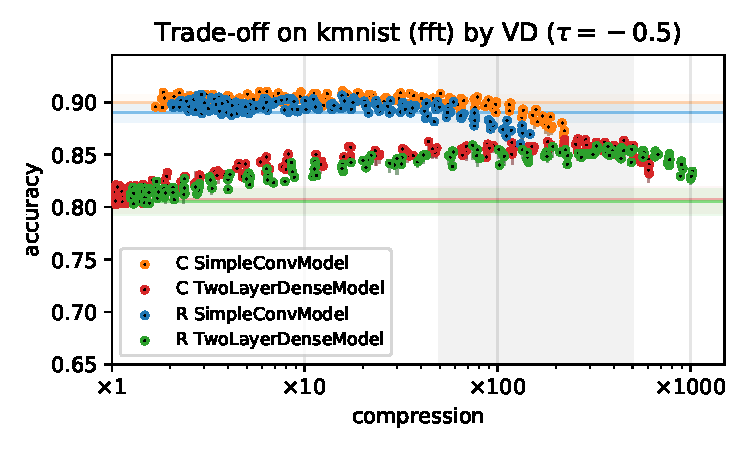
\includegraphics[width=\columnwidth]{figure__mnist-like__trade-off/appendix__VD__kmnist__fft__-0.5.pdf}
  \end{subfigure}%
  \begin{subfigure}[b]{0.5\columnwidth}
    \centering
    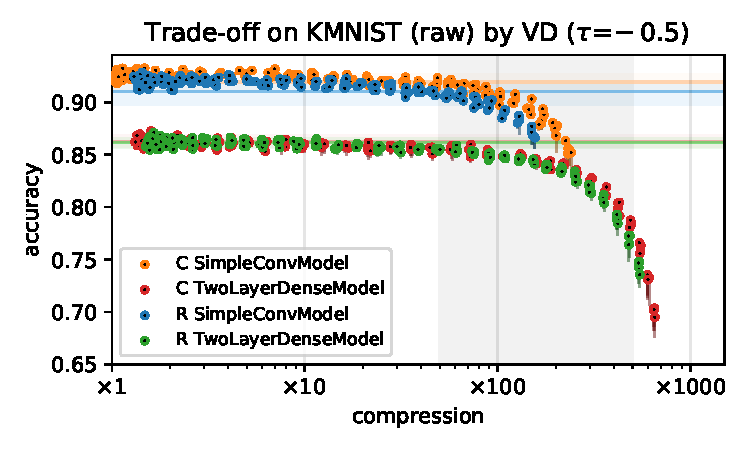
\includegraphics[width=\columnwidth]{figure__mnist-like__trade-off/appendix__VD__kmnist__raw__-0.5.pdf}
  \end{subfigure}
  \caption{%
    \texttt{kmnist}:
      \texttt{fft} (left), \texttt{raw} (right).
      Models on rows 1 \& 2 are incomparable: (left $2\real / \cplx$), (right $\real / \tfrac12\cplx$).
      Rows 3 \& 4 feature $\real / \cplx$ models.
    % VD method for $\real$ and $\cplx$ models using Fourier features.
  }
  % \label{fig:appendix__mnist-like__trade-off__kmnist}
\end{figure}

\begin{figure}[b]
  \centering
  \begin{subfigure}[b]{0.5\columnwidth}
    \centering
    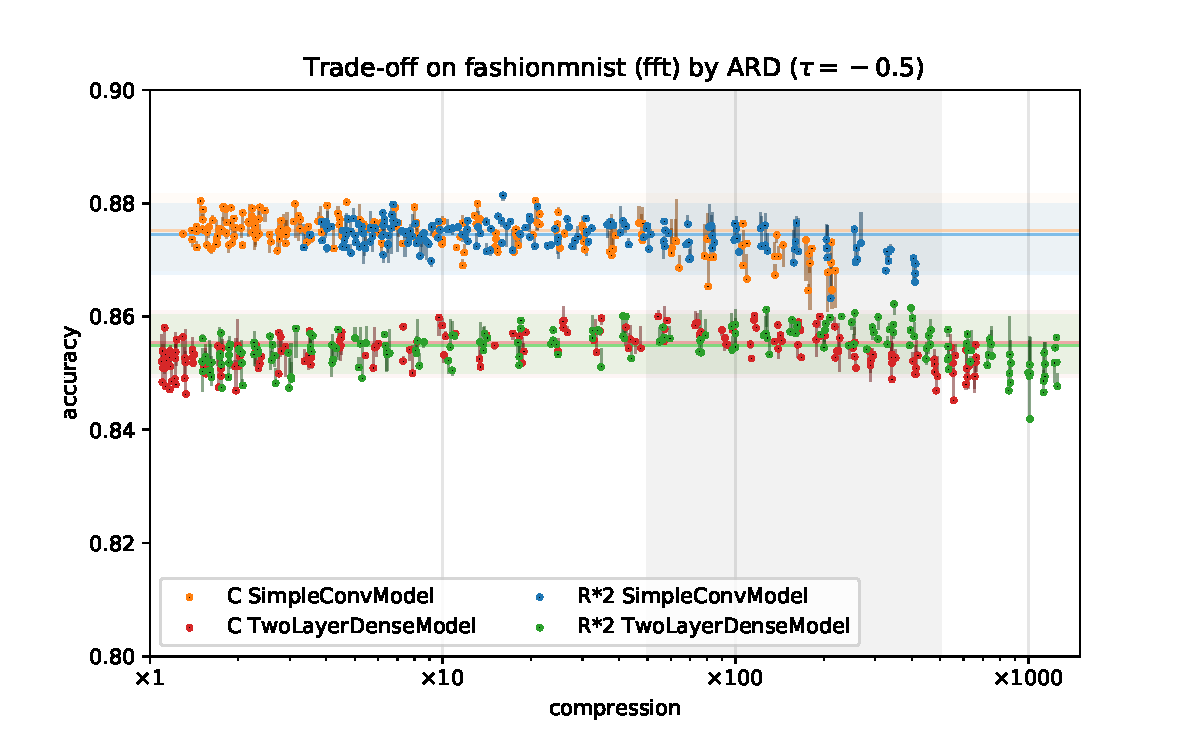
\includegraphics[width=\columnwidth]{figure__mnist-like__trade-off/appendix__cmp__ARD__fashionmnist__fft__-0.5.pdf}
  \end{subfigure}%
  \begin{subfigure}[b]{0.5\columnwidth}
    \centering
    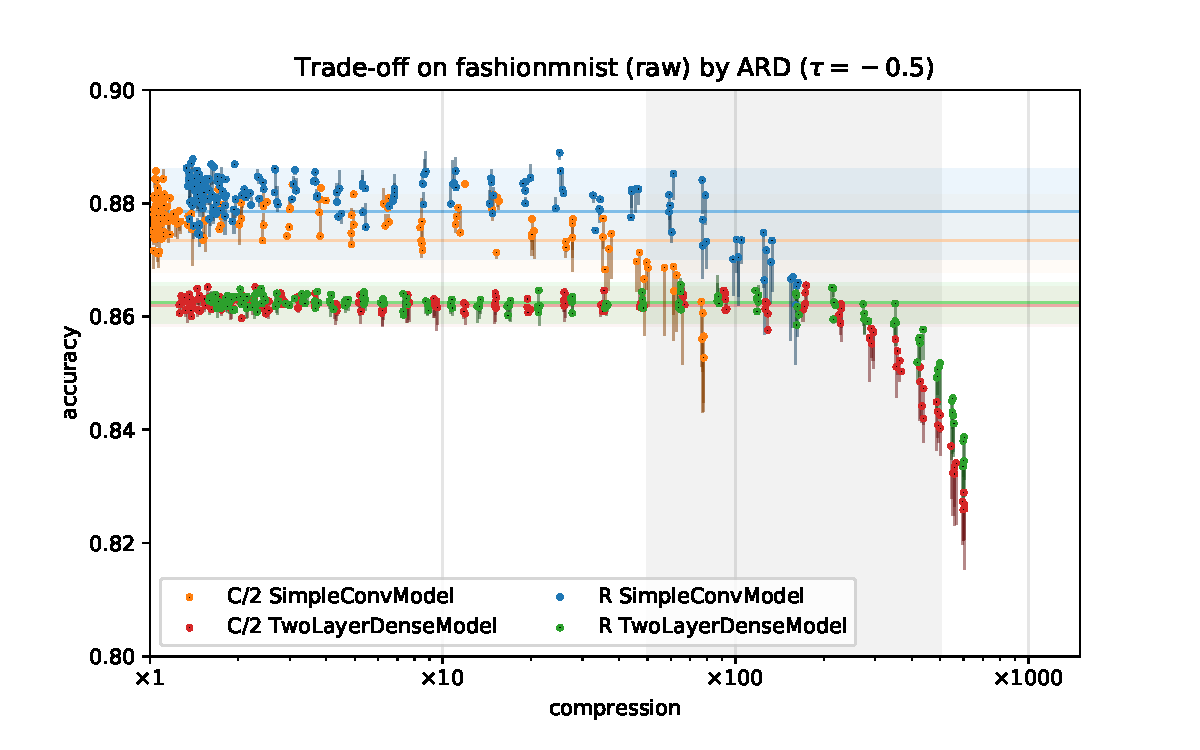
\includegraphics[width=\columnwidth]{figure__mnist-like__trade-off/appendix__cmp__ARD__fashionmnist__raw__-0.5.pdf}
  \end{subfigure} \\%
  \begin{subfigure}[b]{0.5\columnwidth}
    \centering
    % used in main text
    \includegraphics[width=\columnwidth]{figure__mnist-like__trade-off/appendix__ARD__fashionmnist__fft__-0.5.pdf}
  \end{subfigure}%
  \begin{subfigure}[b]{0.5\columnwidth}
    \centering
    \includegraphics[width=\columnwidth]{figure__mnist-like__trade-off/appendix__ARD__fashionmnist__raw__-0.5.pdf}
  \end{subfigure} \\%
  \begin{subfigure}[b]{0.5\columnwidth}
    \centering
    \includegraphics[width=\columnwidth]{figure__mnist-like__trade-off/appendix__cmp__VD__fashionmnist__fft__-0.5.pdf}
  \end{subfigure}%
  \begin{subfigure}[b]{0.5\columnwidth}
    \centering
    \includegraphics[width=\columnwidth]{figure__mnist-like__trade-off/appendix__cmp__VD__fashionmnist__raw__-0.5.pdf}
  \end{subfigure} \\ %
  \begin{subfigure}[b]{0.5\columnwidth}
    \centering
    \includegraphics[width=\columnwidth]{figure__mnist-like__trade-off/appendix__VD__fashionmnist__fft__-0.5.pdf}
  \end{subfigure}%
  \begin{subfigure}[b]{0.5\columnwidth}
    \centering
    \includegraphics[width=\columnwidth]{figure__mnist-like__trade-off/appendix__VD__fashionmnist__raw__-0.5.pdf}
  \end{subfigure}
  \caption{%
    \texttt{fashionmnist}:
      \texttt{fft} (left), \texttt{raw} (right).
      Models on rows 1 \& 3 are incomparable: (left $2\real / \cplx$), (right $\real / \tfrac12\cplx$).
      Rows 2 \& 4 feature $\real / \cplx$ models.
    % ARD method for $\real$ and $\cplx$ models using raw features.
  }
  % \label{fig:appendix__mnist-like__trade-off__fashionmnist}
\end{figure}

\begin{figure}[b]
  \centering
  \begin{subfigure}[b]{0.5\columnwidth}
    \centering
    \includegraphics[width=\columnwidth]{figure__mnist-like__trade-off/appendix__cmp__ARD__mnist__fft__-0.5.pdf}
  \end{subfigure}%
  \begin{subfigure}[b]{0.5\columnwidth}
    \centering
    \includegraphics[width=\columnwidth]{figure__mnist-like__trade-off/appendix__cmp__ARD__mnist__raw__-0.5.pdf}
  \end{subfigure} \\%
  \begin{subfigure}[b]{0.5\columnwidth}
    \centering
    % used in main text
    \includegraphics[width=\columnwidth]{figure__mnist-like__trade-off/appendix__ARD__mnist__fft__-0.5.pdf}
  \end{subfigure}%
  \begin{subfigure}[b]{0.5\columnwidth}
    \centering
    \includegraphics[width=\columnwidth]{figure__mnist-like__trade-off/appendix__ARD__mnist__raw__-0.5.pdf}
  \end{subfigure} \\%
  \begin{subfigure}[b]{0.5\columnwidth}
    \centering
    \includegraphics[width=\columnwidth]{figure__mnist-like__trade-off/appendix__cmp__VD__mnist__fft__-0.5.pdf}
  \end{subfigure}%
  \begin{subfigure}[b]{0.5\columnwidth}
    \centering
    \includegraphics[width=\columnwidth]{figure__mnist-like__trade-off/appendix__cmp__VD__mnist__raw__-0.5.pdf}
  \end{subfigure} \\ %
  \begin{subfigure}[b]{0.5\columnwidth}
    \centering
    \includegraphics[width=\columnwidth]{figure__mnist-like__trade-off/appendix__VD__mnist__fft__-0.5.pdf}
  \end{subfigure}%
  \begin{subfigure}[b]{0.5\columnwidth}
    \centering
    \includegraphics[width=\columnwidth]{figure__mnist-like__trade-off/appendix__VD__mnist__raw__-0.5.pdf}
  \end{subfigure}
  \caption{%
    \texttt{mnist}:
      \texttt{fft} (left), \texttt{raw} (right).
      Models on rows 1 \& 2 are incomparable: (left $2\real / \cplx$), (right $\real / \tfrac12\cplx$).
      Rows 3 \& 4 feature $\real / \cplx$ models.
    % VD method for $\real$ and $\cplx$ models using raw features.
  }
  % \label{fig:appendix__mnist-like__trade-off__mnist}
\end{figure}



\begin{figure}[b]
  \centering
  \begin{subfigure}[b]{0.5\columnwidth}
    \centering
    \includegraphics[width=\columnwidth]{figure__mnist-like__trade-off/appendix__cmp__ARD__emnist_letters__fft__-0.5.pdf}
  \end{subfigure}%
  \begin{subfigure}[b]{0.5\columnwidth}
    \centering
    \includegraphics[width=\columnwidth]{figure__mnist-like__trade-off/appendix__cmp__ARD__emnist_letters__raw__-0.5.pdf}
  \end{subfigure} \\ %
  \begin{subfigure}[b]{0.5\columnwidth}
    \centering
    % used in main text
    \includegraphics[width=\columnwidth]{figure__mnist-like__trade-off/appendix__cmp__ARD__kmnist__fft__-0.5.pdf}
  \end{subfigure}%
  \begin{subfigure}[b]{0.5\columnwidth}
    \centering
    \includegraphics[width=\columnwidth]{figure__mnist-like__trade-off/appendix__cmp__ARD__kmnist__raw__-0.5.pdf}
  \end{subfigure} \\ %
  \begin{subfigure}[b]{0.5\columnwidth}
    \centering
    \includegraphics[width=\columnwidth]{figure__mnist-like__trade-off/appendix__cmp__ARD__fashionmnist__fft__-0.5.pdf}
  \end{subfigure}%
  \begin{subfigure}[b]{0.5\columnwidth}
    \centering
    \includegraphics[width=\columnwidth]{figure__mnist-like__trade-off/appendix__cmp__ARD__fashionmnist__raw__-0.5.pdf}
  \end{subfigure} \\ %
  \begin{subfigure}[b]{0.5\columnwidth}
    \centering
    \includegraphics[width=\columnwidth]{figure__mnist-like__trade-off/appendix__cmp__ARD__mnist__fft__-0.5.pdf}
  \end{subfigure}%
  \begin{subfigure}[b]{0.5\columnwidth}
    \centering
    \includegraphics[width=\columnwidth]{figure__mnist-like__trade-off/appendix__cmp__ARD__mnist__raw__-0.5.pdf}
  \end{subfigure}
  \caption{%
    \texttt{ARD}.
      \texttt{fft} (left $2\real / \cplx$), \texttt{raw} (right $\real / \tfrac12\cplx$).
      Rows from top to bottom: EMNIST-Letters, KMNIST, Fashion-MNIST, MNIST.
    % ARD method for $\real$ and $\cplx$ models using Fourier features.
  }
  % \label{fig:appendix__mnist-like__trade-off__emnist_letters}
\end{figure}

\begin{figure}[b]
  \centering
  \begin{subfigure}[b]{0.5\columnwidth}
    \centering
    \includegraphics[width=\columnwidth]{figure__mnist-like__trade-off/appendix__ARD__emnist_letters__fft__-0.5.pdf}
  \end{subfigure}%
  \begin{subfigure}[b]{0.5\columnwidth}
    \centering
    \includegraphics[width=\columnwidth]{figure__mnist-like__trade-off/appendix__ARD__emnist_letters__raw__-0.5.pdf}
  \end{subfigure} \\ %
  \begin{subfigure}[b]{0.5\columnwidth}
    \centering
    % used in main text
    \includegraphics[width=\columnwidth]{figure__mnist-like__trade-off/appendix__ARD__kmnist__fft__-0.5.pdf}
  \end{subfigure}%
  \begin{subfigure}[b]{0.5\columnwidth}
    \centering
    \includegraphics[width=\columnwidth]{figure__mnist-like__trade-off/appendix__ARD__kmnist__raw__-0.5.pdf}
  \end{subfigure} \\ %
  \begin{subfigure}[b]{0.5\columnwidth}
    \centering
    \includegraphics[width=\columnwidth]{figure__mnist-like__trade-off/appendix__ARD__fashionmnist__fft__-0.5.pdf}
  \end{subfigure}%
  \begin{subfigure}[b]{0.5\columnwidth}
    \centering
    \includegraphics[width=\columnwidth]{figure__mnist-like__trade-off/appendix__ARD__fashionmnist__raw__-0.5.pdf}
  \end{subfigure} \\ %
  \begin{subfigure}[b]{0.5\columnwidth}
    \centering
    \includegraphics[width=\columnwidth]{figure__mnist-like__trade-off/appendix__ARD__mnist__fft__-0.5.pdf}
  \end{subfigure}%
  \begin{subfigure}[b]{0.5\columnwidth}
    \centering
    \includegraphics[width=\columnwidth]{figure__mnist-like__trade-off/appendix__ARD__mnist__raw__-0.5.pdf}
  \end{subfigure}
  \caption{%
    \texttt{ARD} $\real / \cplx$.
      \texttt{fft} (left), \texttt{raw} (right).
      Rows from top to bottom: EMNIST-Letters, KMNIST, Fashion-MNIST, MNIST.
    % VD method for $\real$ and $\cplx$ models using Fourier features.
  }
  % \label{fig:appendix__mnist-like__trade-off__kmnist}
\end{figure}

\begin{figure}[b]
  \centering
  \begin{subfigure}[b]{0.5\columnwidth}
    \centering
    \includegraphics[width=\columnwidth]{figure__mnist-like__trade-off/appendix__cmp__VD__emnist_letters__fft__-0.5.pdf}
  \end{subfigure}%
  \begin{subfigure}[b]{0.5\columnwidth}
    \centering
    \includegraphics[width=\columnwidth]{figure__mnist-like__trade-off/appendix__cmp__VD__emnist_letters__raw__-0.5.pdf}
  \end{subfigure} \\%
  \begin{subfigure}[b]{0.5\columnwidth}
    \centering
    % used in main text
    \includegraphics[width=\columnwidth]{figure__mnist-like__trade-off/appendix__cmp__VD__kmnist__fft__-0.5.pdf}
  \end{subfigure}%
  \begin{subfigure}[b]{0.5\columnwidth}
    \centering
    \includegraphics[width=\columnwidth]{figure__mnist-like__trade-off/appendix__cmp__VD__kmnist__raw__-0.5.pdf}
  \end{subfigure} \\%
  \begin{subfigure}[b]{0.5\columnwidth}
    \centering
    \includegraphics[width=\columnwidth]{figure__mnist-like__trade-off/appendix__cmp__VD__fashionmnist__fft__-0.5.pdf}
  \end{subfigure}%
  \begin{subfigure}[b]{0.5\columnwidth}
    \centering
    \includegraphics[width=\columnwidth]{figure__mnist-like__trade-off/appendix__cmp__VD__fashionmnist__raw__-0.5.pdf}
  \end{subfigure} \\ %
  \begin{subfigure}[b]{0.5\columnwidth}
    \centering
    \includegraphics[width=\columnwidth]{figure__mnist-like__trade-off/appendix__cmp__VD__mnist__fft__-0.5.pdf}
  \end{subfigure}%
  \begin{subfigure}[b]{0.5\columnwidth}
    \centering
    \includegraphics[width=\columnwidth]{figure__mnist-like__trade-off/appendix__cmp__VD__mnist__raw__-0.5.pdf}
  \end{subfigure}
  \caption{%
    \texttt{VD}
      \texttt{fft} (left $2\real / \cplx$), \texttt{raw} (right $\real / \tfrac12\cplx$).
      Rows from top to bottom: EMNIST-Letters, KMNIST, Fashion-MNIST, MNIST.
    % ARD method for $\real$ and $\cplx$ models using raw features.
  }
  % \label{fig:appendix__mnist-like__trade-off__fashionmnist}
\end{figure}

\begin{figure}[b]
  \centering
  \begin{subfigure}[b]{0.5\columnwidth}
    \centering
    \includegraphics[width=\columnwidth]{figure__mnist-like__trade-off/appendix__VD__emnist_letters__fft__-0.5.pdf}
  \end{subfigure}%
  \begin{subfigure}[b]{0.5\columnwidth}
    \centering
    \includegraphics[width=\columnwidth]{figure__mnist-like__trade-off/appendix__VD__emnist_letters__raw__-0.5.pdf}
  \end{subfigure} \\%
  \begin{subfigure}[b]{0.5\columnwidth}
    \centering
    % used in main text
    \includegraphics[width=\columnwidth]{figure__mnist-like__trade-off/appendix__VD__kmnist__fft__-0.5.pdf}
  \end{subfigure}%
  \begin{subfigure}[b]{0.5\columnwidth}
    \centering
    \includegraphics[width=\columnwidth]{figure__mnist-like__trade-off/appendix__VD__kmnist__raw__-0.5.pdf}
  \end{subfigure} \\%
  \begin{subfigure}[b]{0.5\columnwidth}
    \centering
    \includegraphics[width=\columnwidth]{figure__mnist-like__trade-off/appendix__VD__fashionmnist__fft__-0.5.pdf}
  \end{subfigure}%
  \begin{subfigure}[b]{0.5\columnwidth}
    \centering
    \includegraphics[width=\columnwidth]{figure__mnist-like__trade-off/appendix__VD__fashionmnist__raw__-0.5.pdf}
  \end{subfigure} \\ %
  \begin{subfigure}[b]{0.5\columnwidth}
    \centering
    \includegraphics[width=\columnwidth]{figure__mnist-like__trade-off/appendix__VD__mnist__fft__-0.5.pdf}
  \end{subfigure}%
  \begin{subfigure}[b]{0.5\columnwidth}
    \centering
    \includegraphics[width=\columnwidth]{figure__mnist-like__trade-off/appendix__VD__mnist__raw__-0.5.pdf}
  \end{subfigure}
  \caption{%
    \texttt{VD} $\real / \cplx$.
      \texttt{fft} (left), \texttt{raw} (right).
      Rows from top to bottom: EMNIST-Letters, KMNIST, Fashion-MNIST, MNIST.
    % VD method for $\real$ and $\cplx$ models using raw features.
  }
  % \label{fig:appendix__mnist-like__trade-off__mnist}
\end{figure}

\end{document}
